
\chapter{加速计算的原理以及实现}
    \indent 在本章中我们希望能够简化积分核值的计算过程。 如同~Ando(2016)~的工作,我们将积分核的计算随着时间的变化分为了三个区域,即初始区,传播区,稳定区,如图2.1所示。从公式上 我们可以对初始区和稳定区积分核的计算公式进行简化,利用简化后的计算公式,我们能够以更高的效率对积分核进行计算。同时,这样的分区也对应了相应的物理性质,这样能够帮助我们更好的理解破裂的过程。
	\section{计算的基本公式与符号说明}
   \indent 积分核的计算公式基于~Tada and Madariaga(2001)~的结果, $\Delta t$~时间内单元滑动速率的积分核由(\ref{con:tandm})式给出,
        \begin{align} \label{con:tandm}
              K_{ij/k}(\textbf{z},t)=L_{ij/k}(\textbf{z},t+\Delta t)-L_{ij/k}(\textbf{z},t)
         \end{align}
    其中$L$表示单元滑动速率在~0~到无穷的积分,$K$为$\Delta t$时间内单元滑动速率的积分,$\textbf{z}$为空间上的坐标。这里我们采用~Feng and Zhang(2017)~的采用三角形离散化方案得到的计算结果。我们想要计算通过坐标变换后,三点坐标分别为$A(a_{1},a_{2},0)$,$B(b_{1},b_{2},0)$,$C(c_{1},c_{2},0)$的三角形在接收点$R(x_{1},x_{2},x_{3})$处的应力响应。得到的结果中~$L_{31/1}$~ 的表达式为公式~(\ref{con:L311})~所示
        \begin{align} \notag
          2\pi L_{31/1} &= \sum^{abc}([-2p^{3}c_{L}tf_{1}(b_{1}-a_{1},x_{1}-b_{1},y_{1},y_{2}) + 2c_{T}^{3}t^{3}f_{2}(b_{1} - a_{1},x_{1}-b_{1},y_{1},y_{2})\\
         & \notag +  6p^{3}c_{L}tx_{3}^{2}f_{2}(b_{1} - a_{1},x_{1} - b_{1},y_{1},y_{2})- 10c_{T}^{3}t^{3}x_{3}^{2}f_{3}(b_{1}-a_{1},x_{1}-b_{1},y_{1},y_{2})\\
         &\notag + 2c_{T}tf_{1}(b_{1}-a_{1},x_{1}-b_{1},z_{1},z_{2}) - 2c_{T}^{3}t^{3}f_{2}(b_{1}-a_{1},x_{1}-b_{1},z_{1},z_{2})\\
         &\notag - 6c_{T}tx_{3}^{2}f_{2}(b_{1}-a_{1},x_{1}-b_{1},z_{1},z_{2})+ 10c_{T}^{3}t^{3}x_{3}^{2}f_{3}(b_{1}-a_{1},x_{1}-b_{1},z_{1},z_{2})](a_{2}-b_{2}) \\
         & + c_{T}t(b_{1}-a_{1})f_{1}(b_{2}-a_{2},x_{2}-b_{2},z_{1},z_{2})  ) + E(c_{L})\label{con:L311}
         \end{align}
         
        \noindent $c_{L}$~表示~P~波波速,$c_{T}$~表示~S~波波速,$\sum^{abc}$表示对~$a_{1}$,$a_{2}$,$b_{1}$,$b_{2}$,$c_{1}$,$c_{2}$~的循环求和,$f_{i}$~的详细表达式以及相关不定积分如何取值的讨论见附录B所示。



    \section{积分核加速计算}

    \indent 由附录B对于定积分上下限的讨论可知,定积分的上下限取值存在不同的情况。由于定积分的取值不同,得到的积分核形式也不同。当定积分上下限的取值是确定的,对应积分核的形式应当也是固定的。同时,我们作出积分核的值随时间的变化图(如图~\ref{fig:yinglichuanbotuxiang}~所示),可知在$t_f$时刻之前,三角形单元对接收点的影响为~0,在~$t_{c}$~时刻之后积分核值为一稳定值。初始区和稳定区的积分核的值为固定的,然而这个部分的计算却占据了计算成本的大部分,因此简化这两个区域的计算就显得很重要。我们可以通过计算到时来判断应力影响到达的位置,通过各个区域的临界到时对积分核的计算进行分区,然后在不同区域中采取不同的优化策略以达到提高计算效率的目的。
  

\begin{figure}[ht]
  \centering
  \begin{subfigure}[b]{0.45\linewidth}
    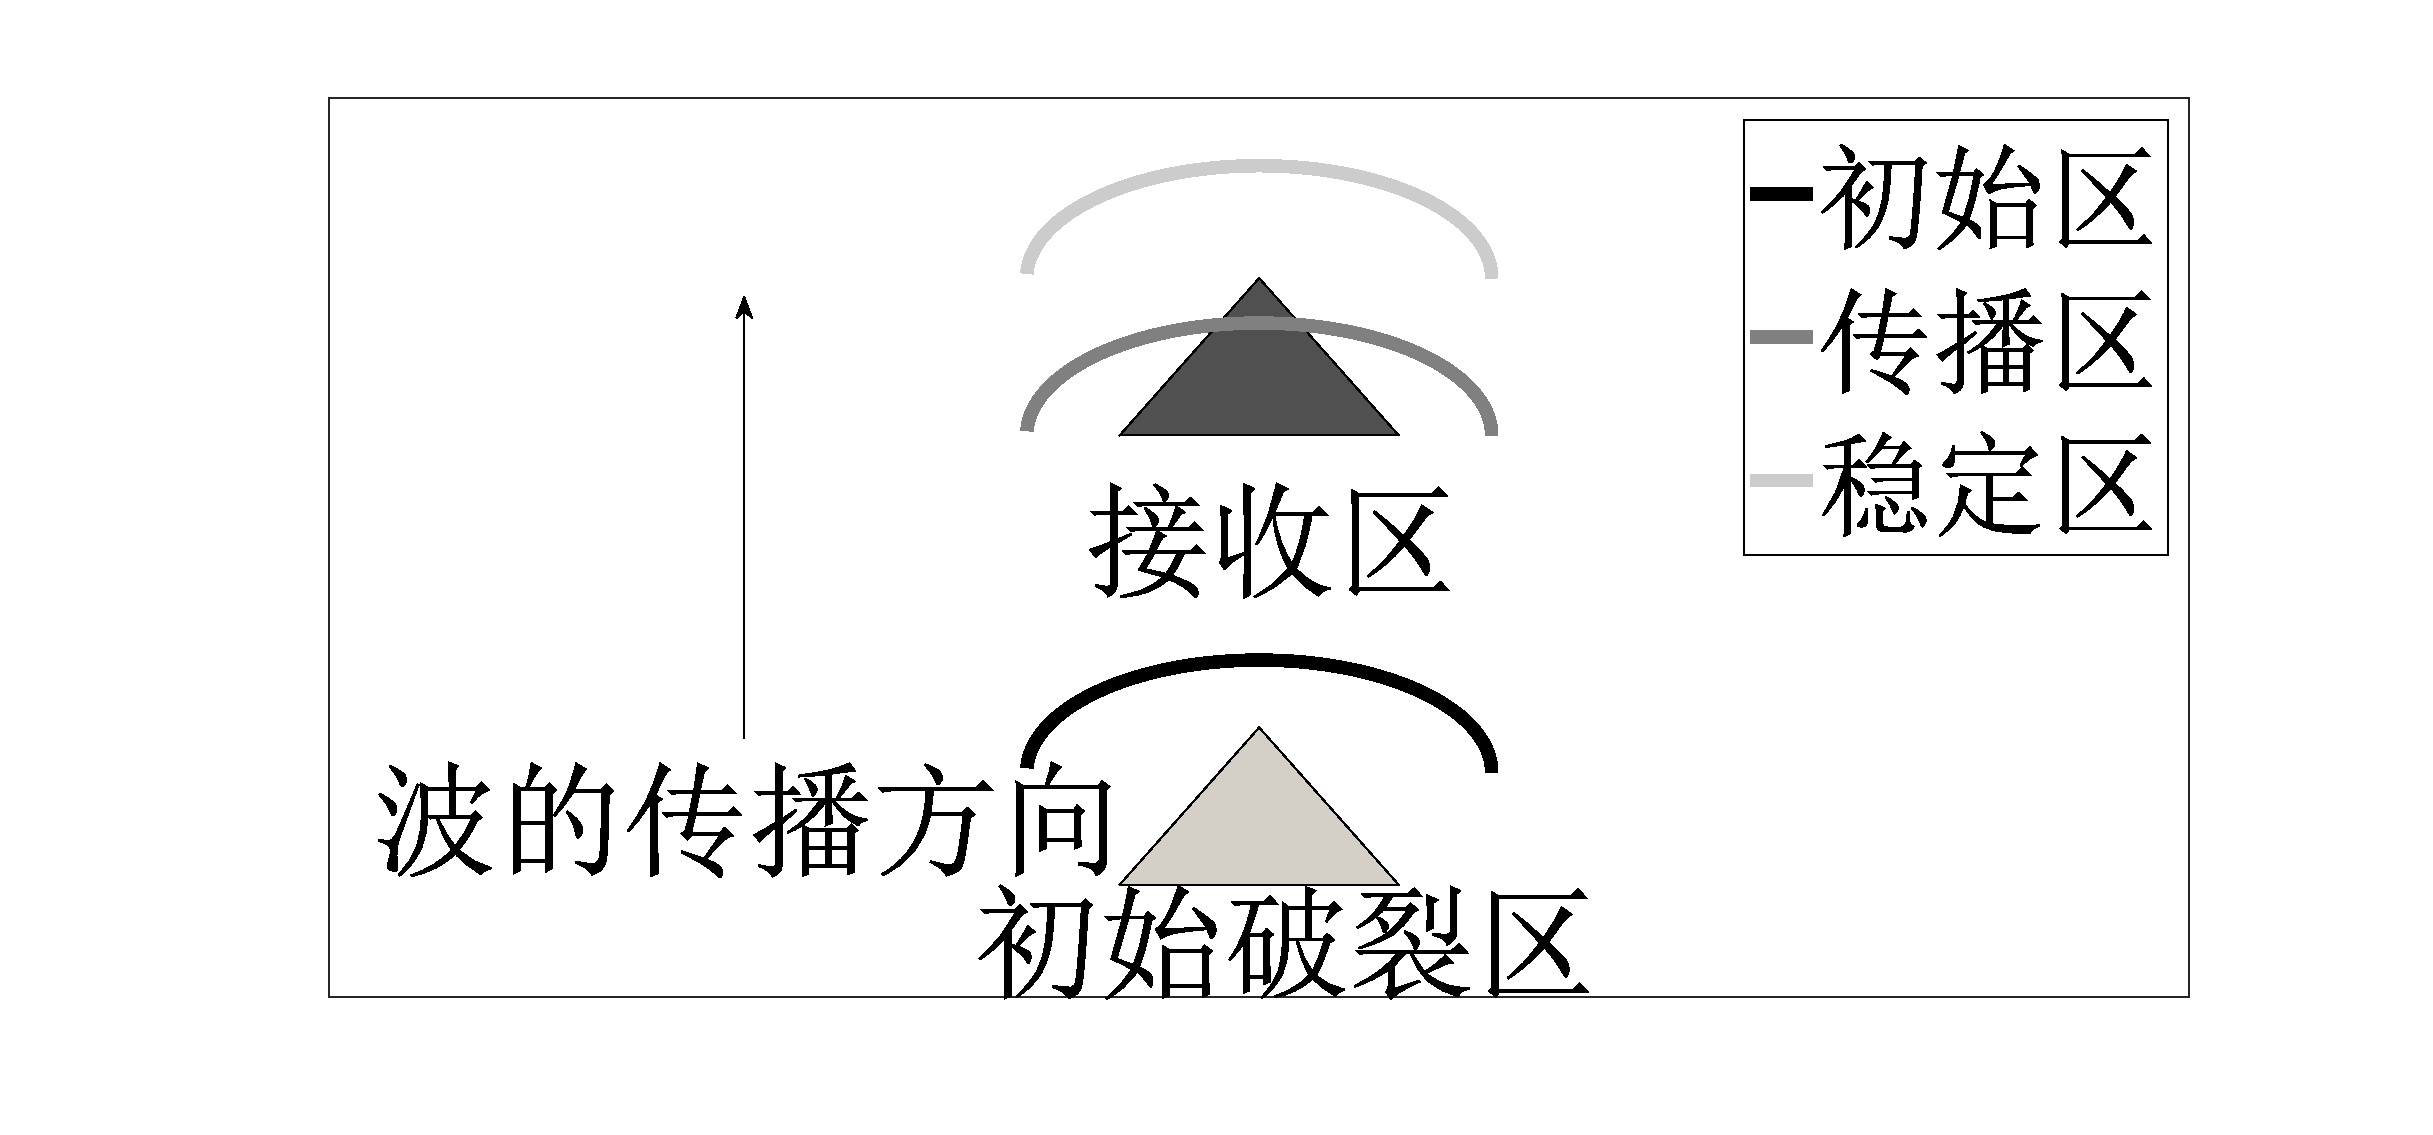
\includegraphics[width=\linewidth]{img/model_1.eps}
    \caption{应力传模型}\label{fig:yinglimoxin}
  \end{subfigure}
  \begin{subfigure}[b]{0.45\linewidth}
    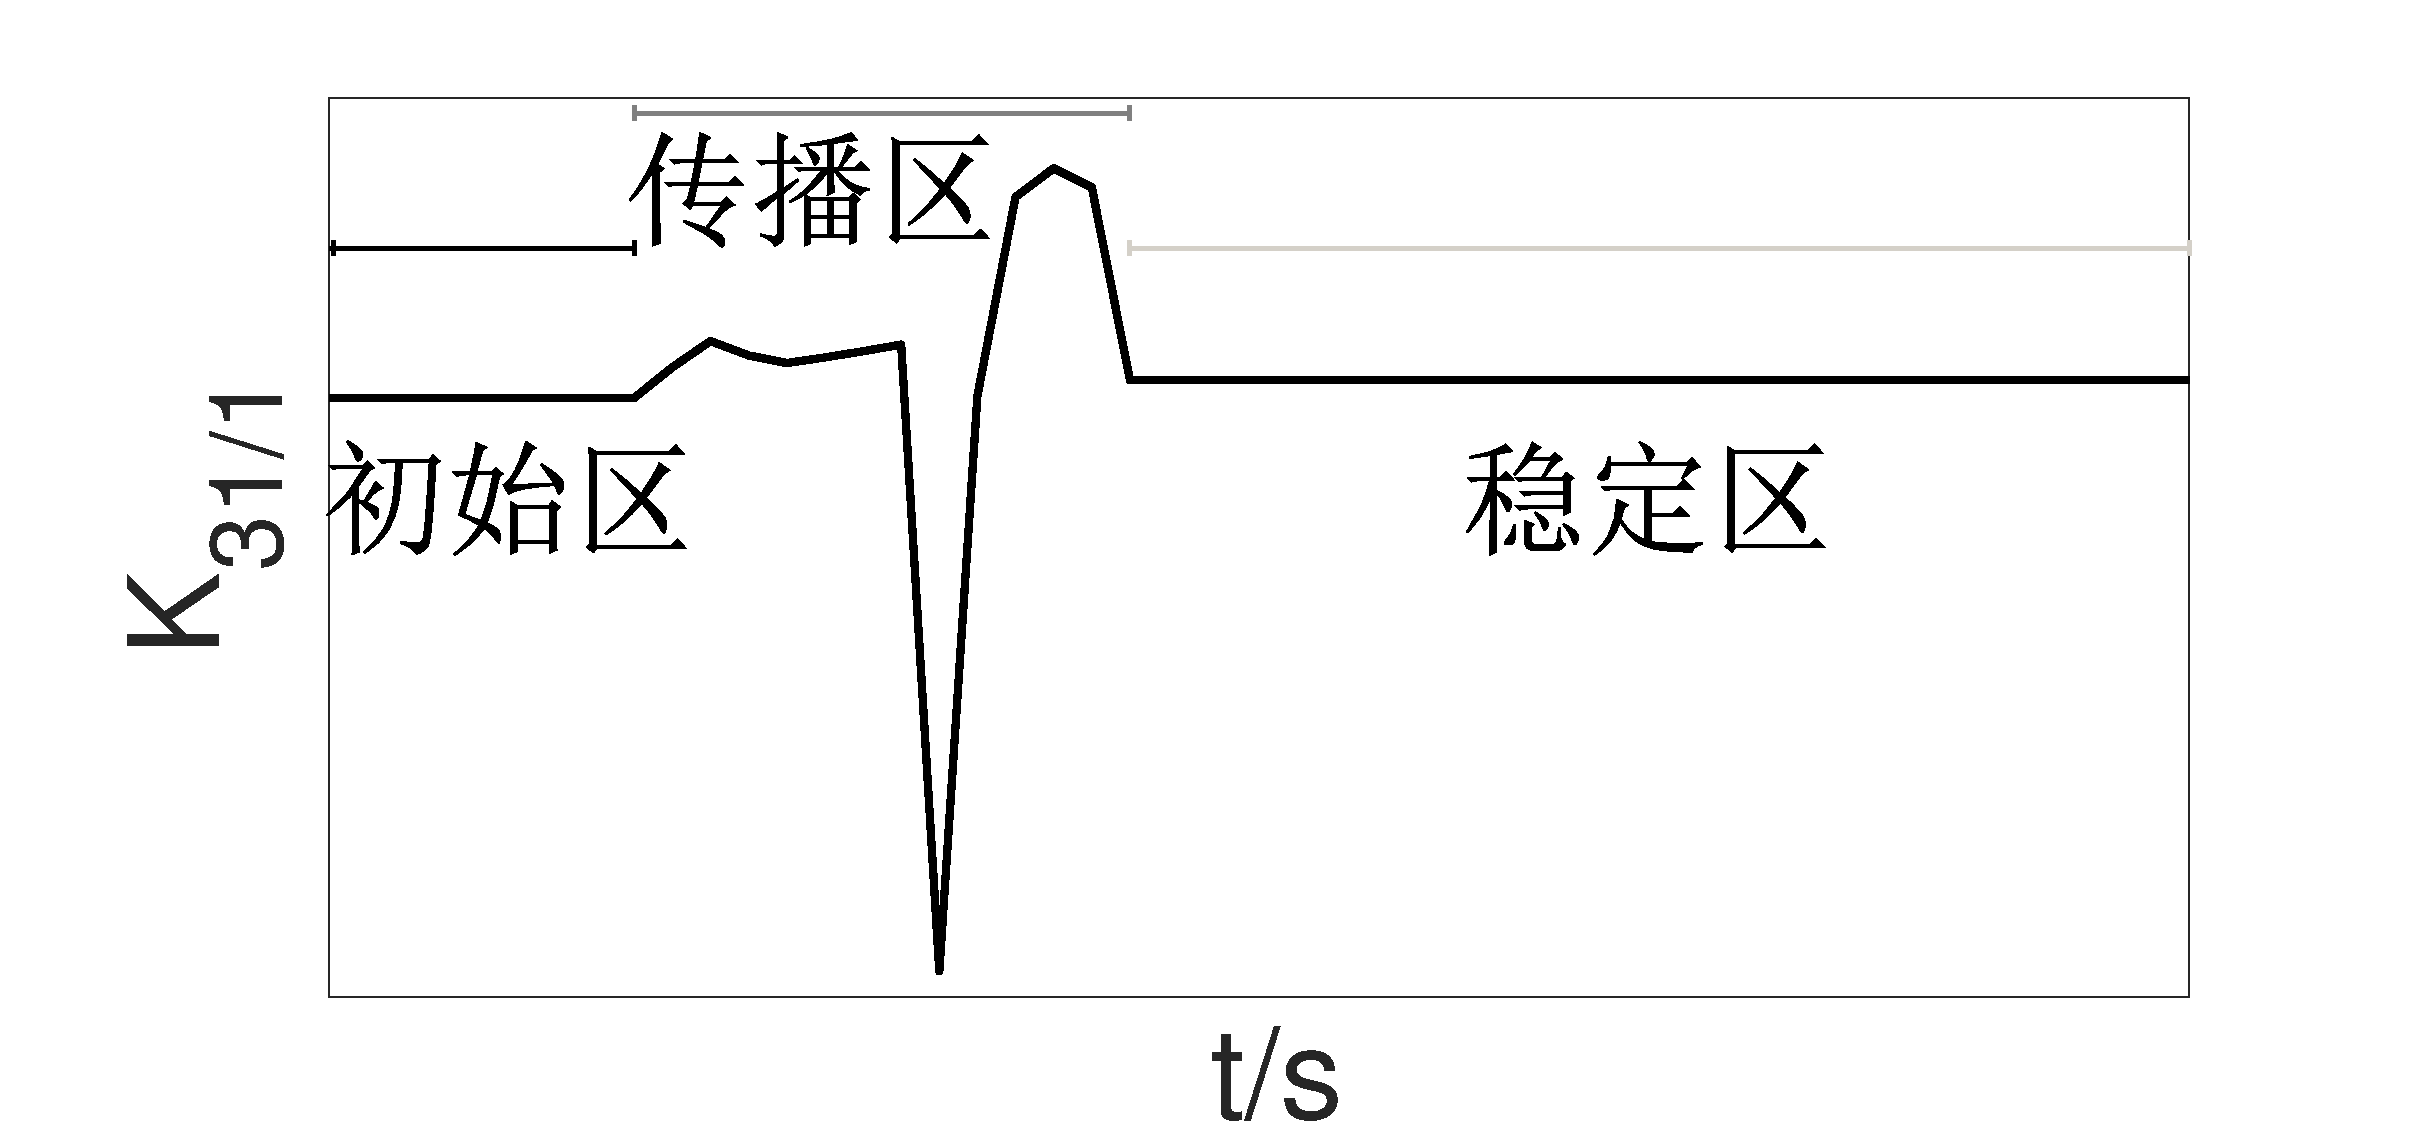
\includegraphics[width=\linewidth]{img/model_2.eps}
    \caption{应力影响传播图像}\label{fig:yinglichuanbotuxiang}
  \end{subfigure}
  \caption{应力传播分区图}
\end{figure}

 \subsection{对初始区积分核计算的简化}
        如图~2.1(a)~所示,当应力的传播未到达影响接收区,此时对应初始区的情况,即此时~P~波和~S~波波前,并未达到其影响的单元。可以得到,对于~P~波的情况,$y_1=0$,$y_2=0$。 对于~S~ 波的情况,$z_1=0$,$z_2=0$。这里,$y_1$,$y_2$,$z_1$,$z_2$的含义见公式~(\ref{con:def-sxxian1}), (\ref{con:def-sxxian2})~中的积分上下限。因此代入计算公式可得
		\begin{equation}
			    	L_{311} = 0 
	     \end{equation}
 \noindent 代入公式~(\ref{con:tandm}),可以求得对应的的积分核为
\begin{equation}
    K_{311} =0 
\end{equation}
为判断地震波是否到达初始区,我们需要求出最小到时$T_{\min}$,我们便可以认为在最小到时之前积分核都为~0。由于~P~波波速大于~S~波,因此我们只需要求出~P~波的最小到时即可。问题转化为如何求点到三角形区域的最短距离。进步一问题转化为点到三角形三边,也就是到求点到三条线段的最小距离。对于点到线段的距离,可以利用投影法进行求解。如图所示,点~P~与线段~AB~的位置关系一共存在三种情况:\\
1.	点~P~在线段~AB~的延长线。此时满足$|PA| = |AB|+|PB|$ (或者 $|PB| = |AB|+|PA|$) 。 此时点到线段的最短距离为$|PB|$(或者$|PA|$)。\\
2.	点~P~的投影在线段~AB~的延长线上,此时满足 $|PA|^2 > | AB |^2 +|PB|^2$( 或者$|PA|^2 > | AB |^2 +|PB|^2$) 。此时点到线段的最短距离为$|PB|$(或者$|PA|$)。\\
3.	点~P~的投影在线段~AB~上。此时需要利用公式~(\ref{con:hl})~计算三角形面积
\begin{equation}
    S = \sqrt{p(p-a)(p-b)(p-c)}  \label{con:hl}
\end{equation} 其中~$p$~为三角形周长的一半,$a$,$b$,$c$~为三角形三边的长度。则点到线段的最短距离为以~AB~ 边为底的高$S/|AB|$。对三角形区域,求出接收点到其的最短距离后,可以求得最小到时$T_{\min} = r/c_{L}$。而对于$t<T_{\min}$ 的情况,积分核$L_{311}$的值为~0。因此对于时间小于最小到时的情况,这部分积分核的值,我们可以不予计算。
\subsection{对稳定区积分核计算的简化}
        \indent 如图~\ref{fig:yinglichuanbotuxiang}~中稳定区所示,
此时对图~\ref{fig:yinglimoxin}~蓝色区域的情况,即此时~P~波和~S~波波前都已经传过影响单元。对于这种情况,对于P波的情况~$y_1=0$,$ y_2 = 1$,对于~S~ 波的情况~$z_1 =0$,$z_2 =1$。代入积分核的计算公式可得
	\begin{equation}
     L_{311} =L_{t}t + E(c_T)
	\end{equation}
\begin{align}\notag
L_{t} &=\sum^{abc}( [-2 p ^3c_{L}tf_1(b_{1}-a_{1},x_{1}-b_{1},0,1) + 6p^3c_{L}tx^{2}_{3}f_{2}(b_{1}-a_{1},x_{1}-b_{1},0,1) \\
\notag
&+ 2c_{T}tf_{1}(b_{1}-a_{1},x_{1}-b_{1},0,1) -6c_{T}tx^{2}_{3}f_{2}(b_{1}-a_{1},x_{1}-b_{1},0,1)](a_{2}- b_{2})\\
&+ c_{T}t(b_{1}-a_{1})f_{1}(b_{2}-a_{2},x_{2}-b_{2},0,1))\notag \label{con:Lt}
\end{align}

\noindent 其中,$L_{t}$的表达式如公式~(\ref{con:Lt})~所示。在到达稳定区后,$L_{311}$~所有的时间的高阶项全部都消去了,只剩下时间的一次项和与时间无关的项。代入到积分核计算公式,可以得到
\begin{equation}
    K_{311} = L_{t} \rm{d}t
\end{equation} 
其中~$K_{311}$~为一个与时间无关的常量。因此只要找到了地震波达到稳定区的到时,那么在稳定区中,我们都可以只计算并储存刚好到达稳定区时的积分核值,而对于其后的积分核都不予计算。由于~S~波波速小于~P~波波速,只用考虑~S~波到达稳定区的临界到时即可。问题转化为,求初始破裂单元到其影响单元的最大距离。而该问题又可以转化为,求解影响单元到初始破裂的三角形单元的三个顶点的最大距离。求出最大距离~$R_{\max}$~后,稳定区临界到时~$t_c = R_{\max} / c_T$。在稳定区临界到时之后,积分核不会变化,我们不用对该时刻之后的积分核进行计算,从而达到加速的目的。
    \section{加速计算效率与正确性检验}
\indent 在前面的内容中,我们通过波的到时对积分核的计算进行了分区,并在初始区和稳定区对积分核的计算进行了简化以达到加速计算的目的。为确定我们加速计算方案的效率并验证该方案的正确性,我们需要与~Feng and Zhang(2017)~的结果进行数值验证。我们选取四个三角形单元,其三点的坐标分别为如图~\ref{fig:model-4}~所示。
\begin{figure}[H]
    \centerin
   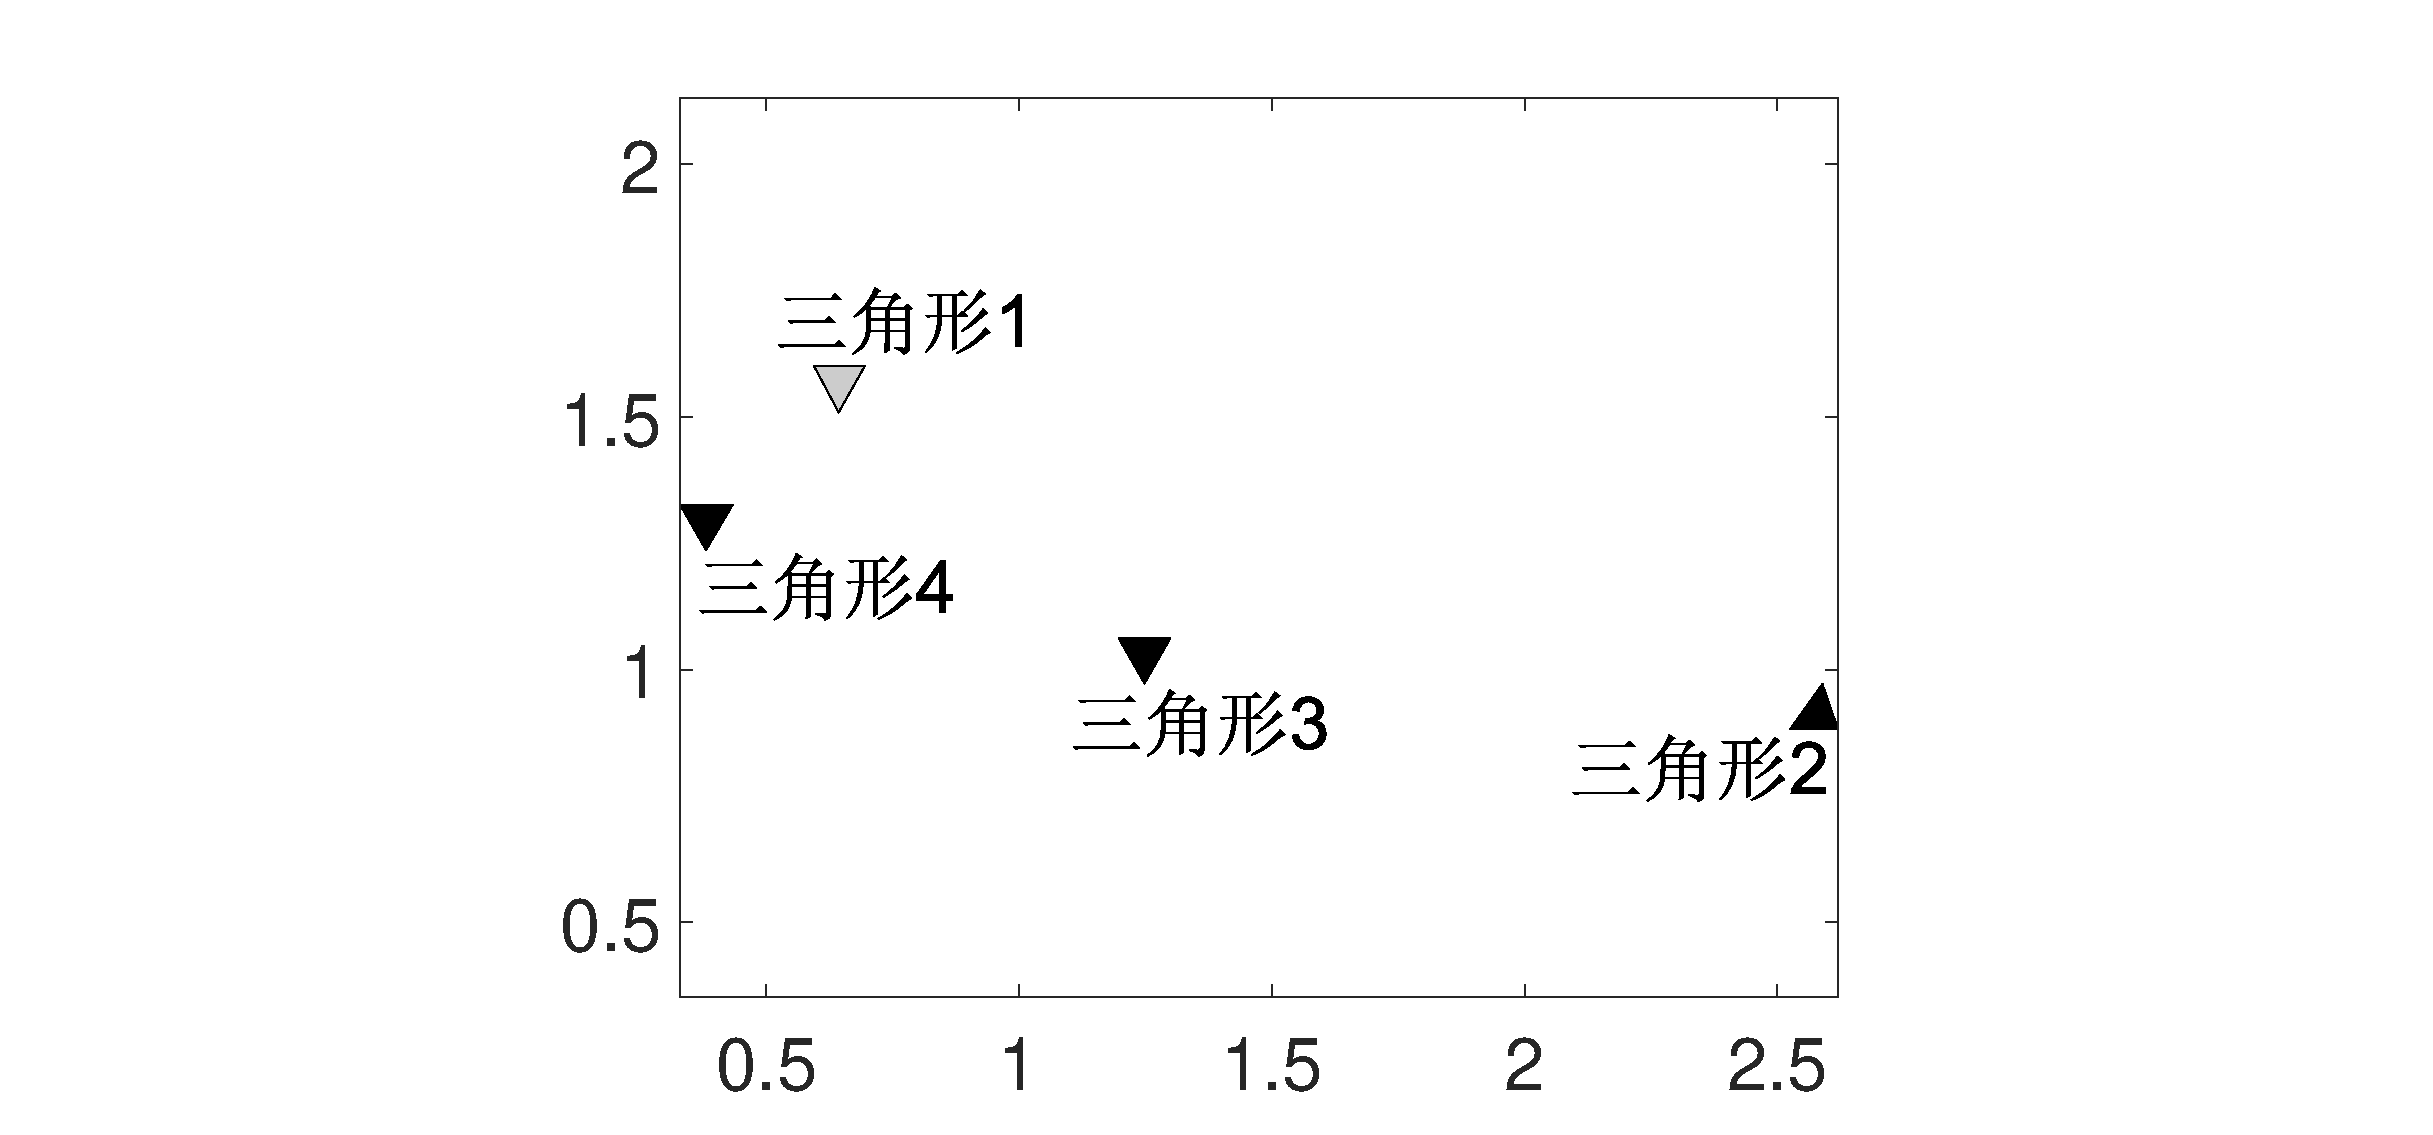
\includegraphics[trim = 0mm 0mm 10mm 0mm, clip=true,width=0.98\linewidth]{img/model.eps}
    \caption{正确性检验模型图} \label{fig:model-4}
  \end{figure}
其中三角形~1~为初始破裂单元,我们计算其对自身以及对其他三个单元的积分核值。P~波波速为~$c_{L} = 5.6~{\rm{km/s}}$,S波波速为~$c_{T} = 3.23~{\rm{km/s}}$。一共计算~50~个时间步。我们采用~Matlab~编程,将两种方法计算得到的积分核值进行比较,结果如图\ref{fig:demenstrate}所示。
%\begin{figure}[htb]  
 % \centering
  %\subfigure[]{
  %\label{fig.1}
  % 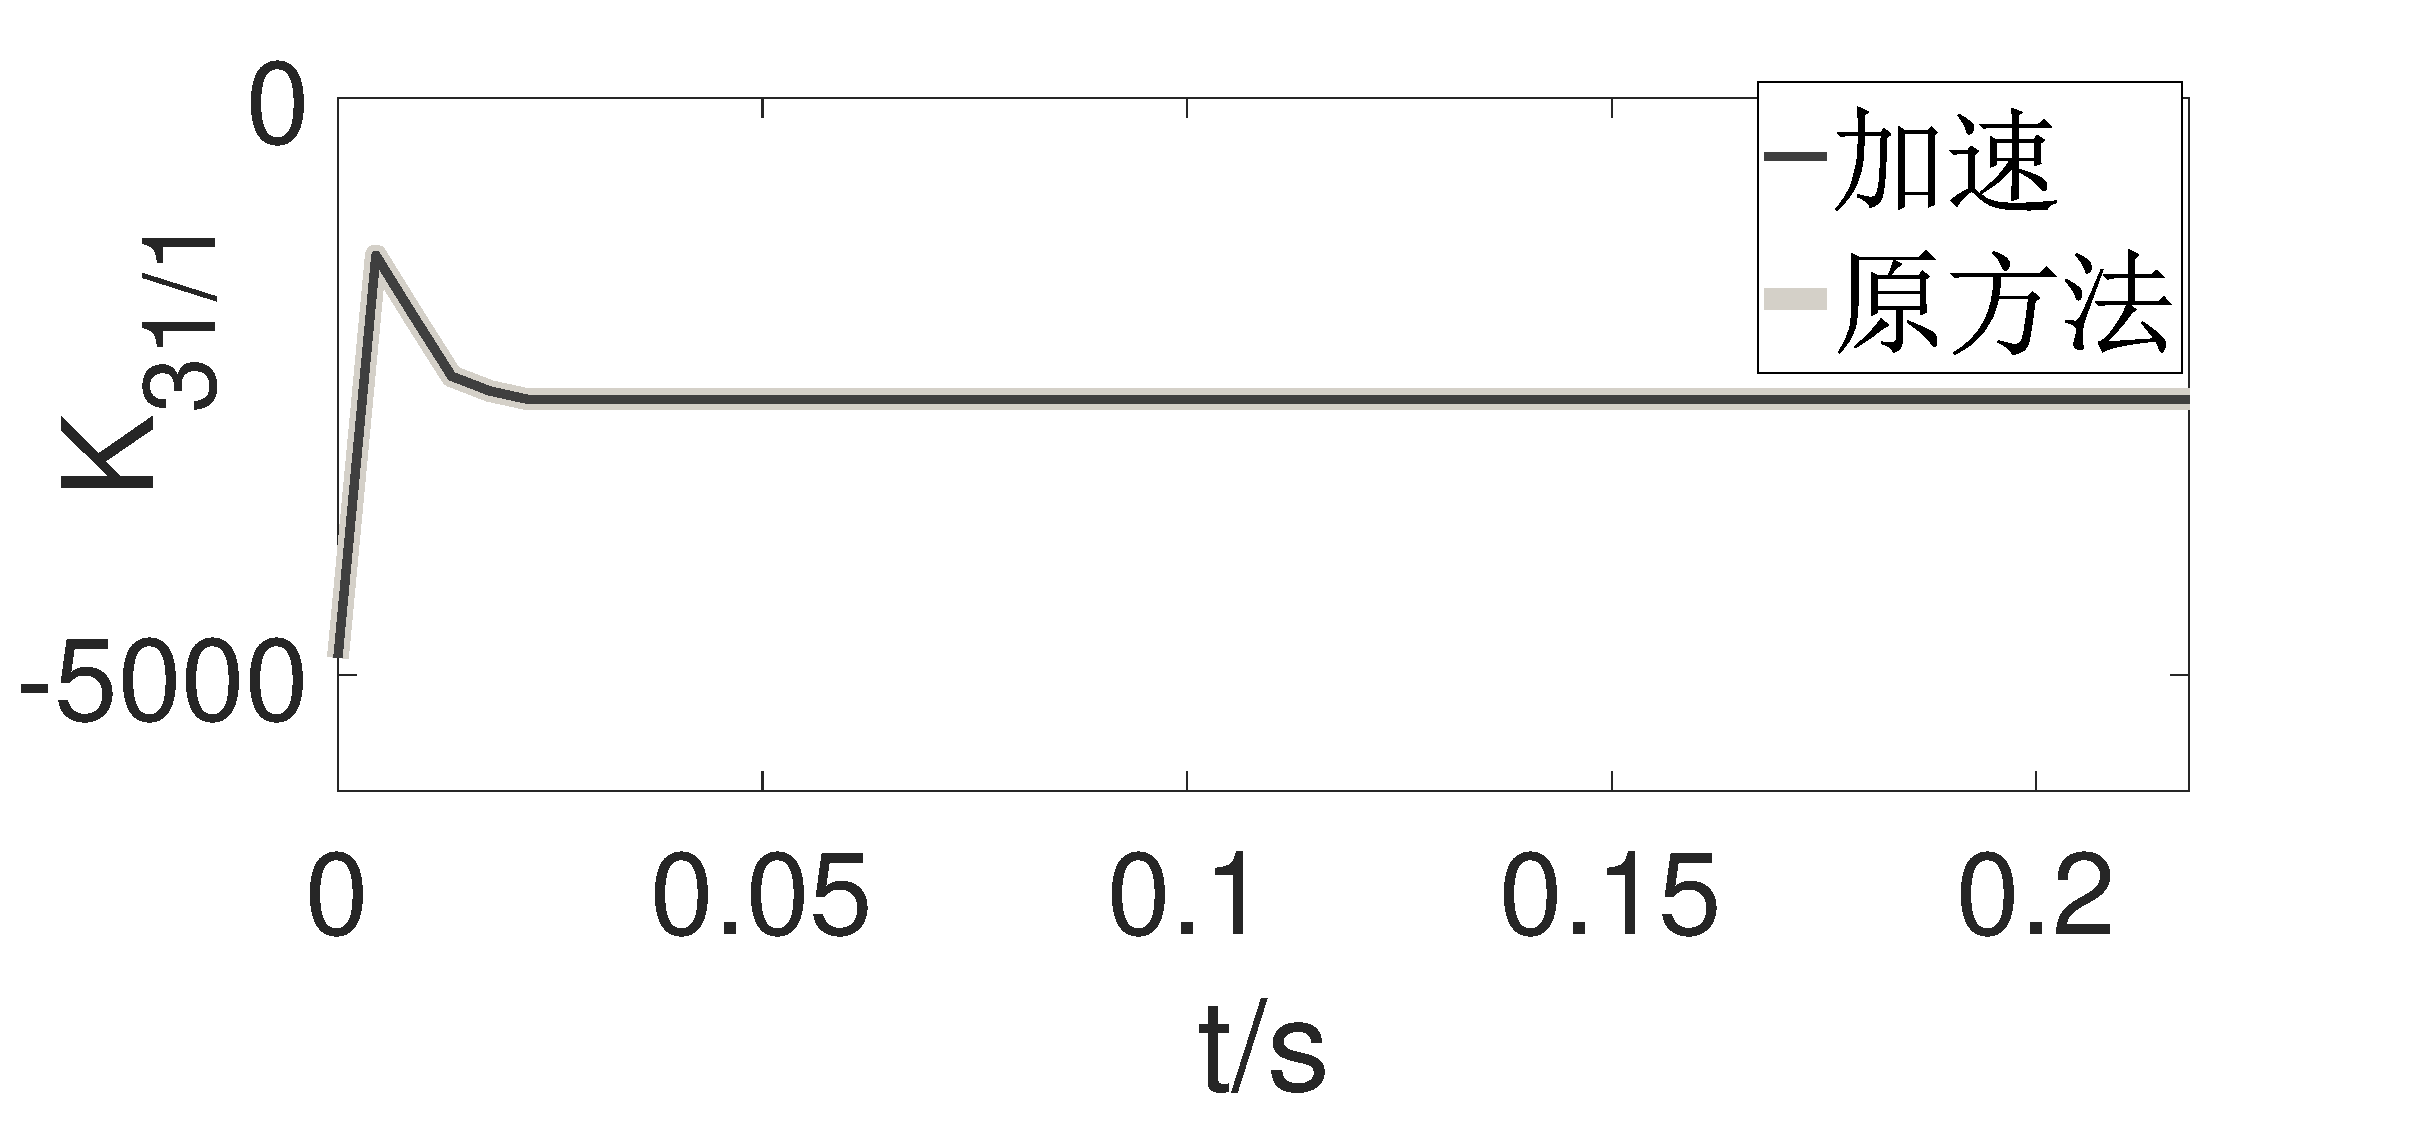
\includegraphics[width=0.5\linewidth]{L311_1_1.eps}}
  % \subfigure[]{
  % 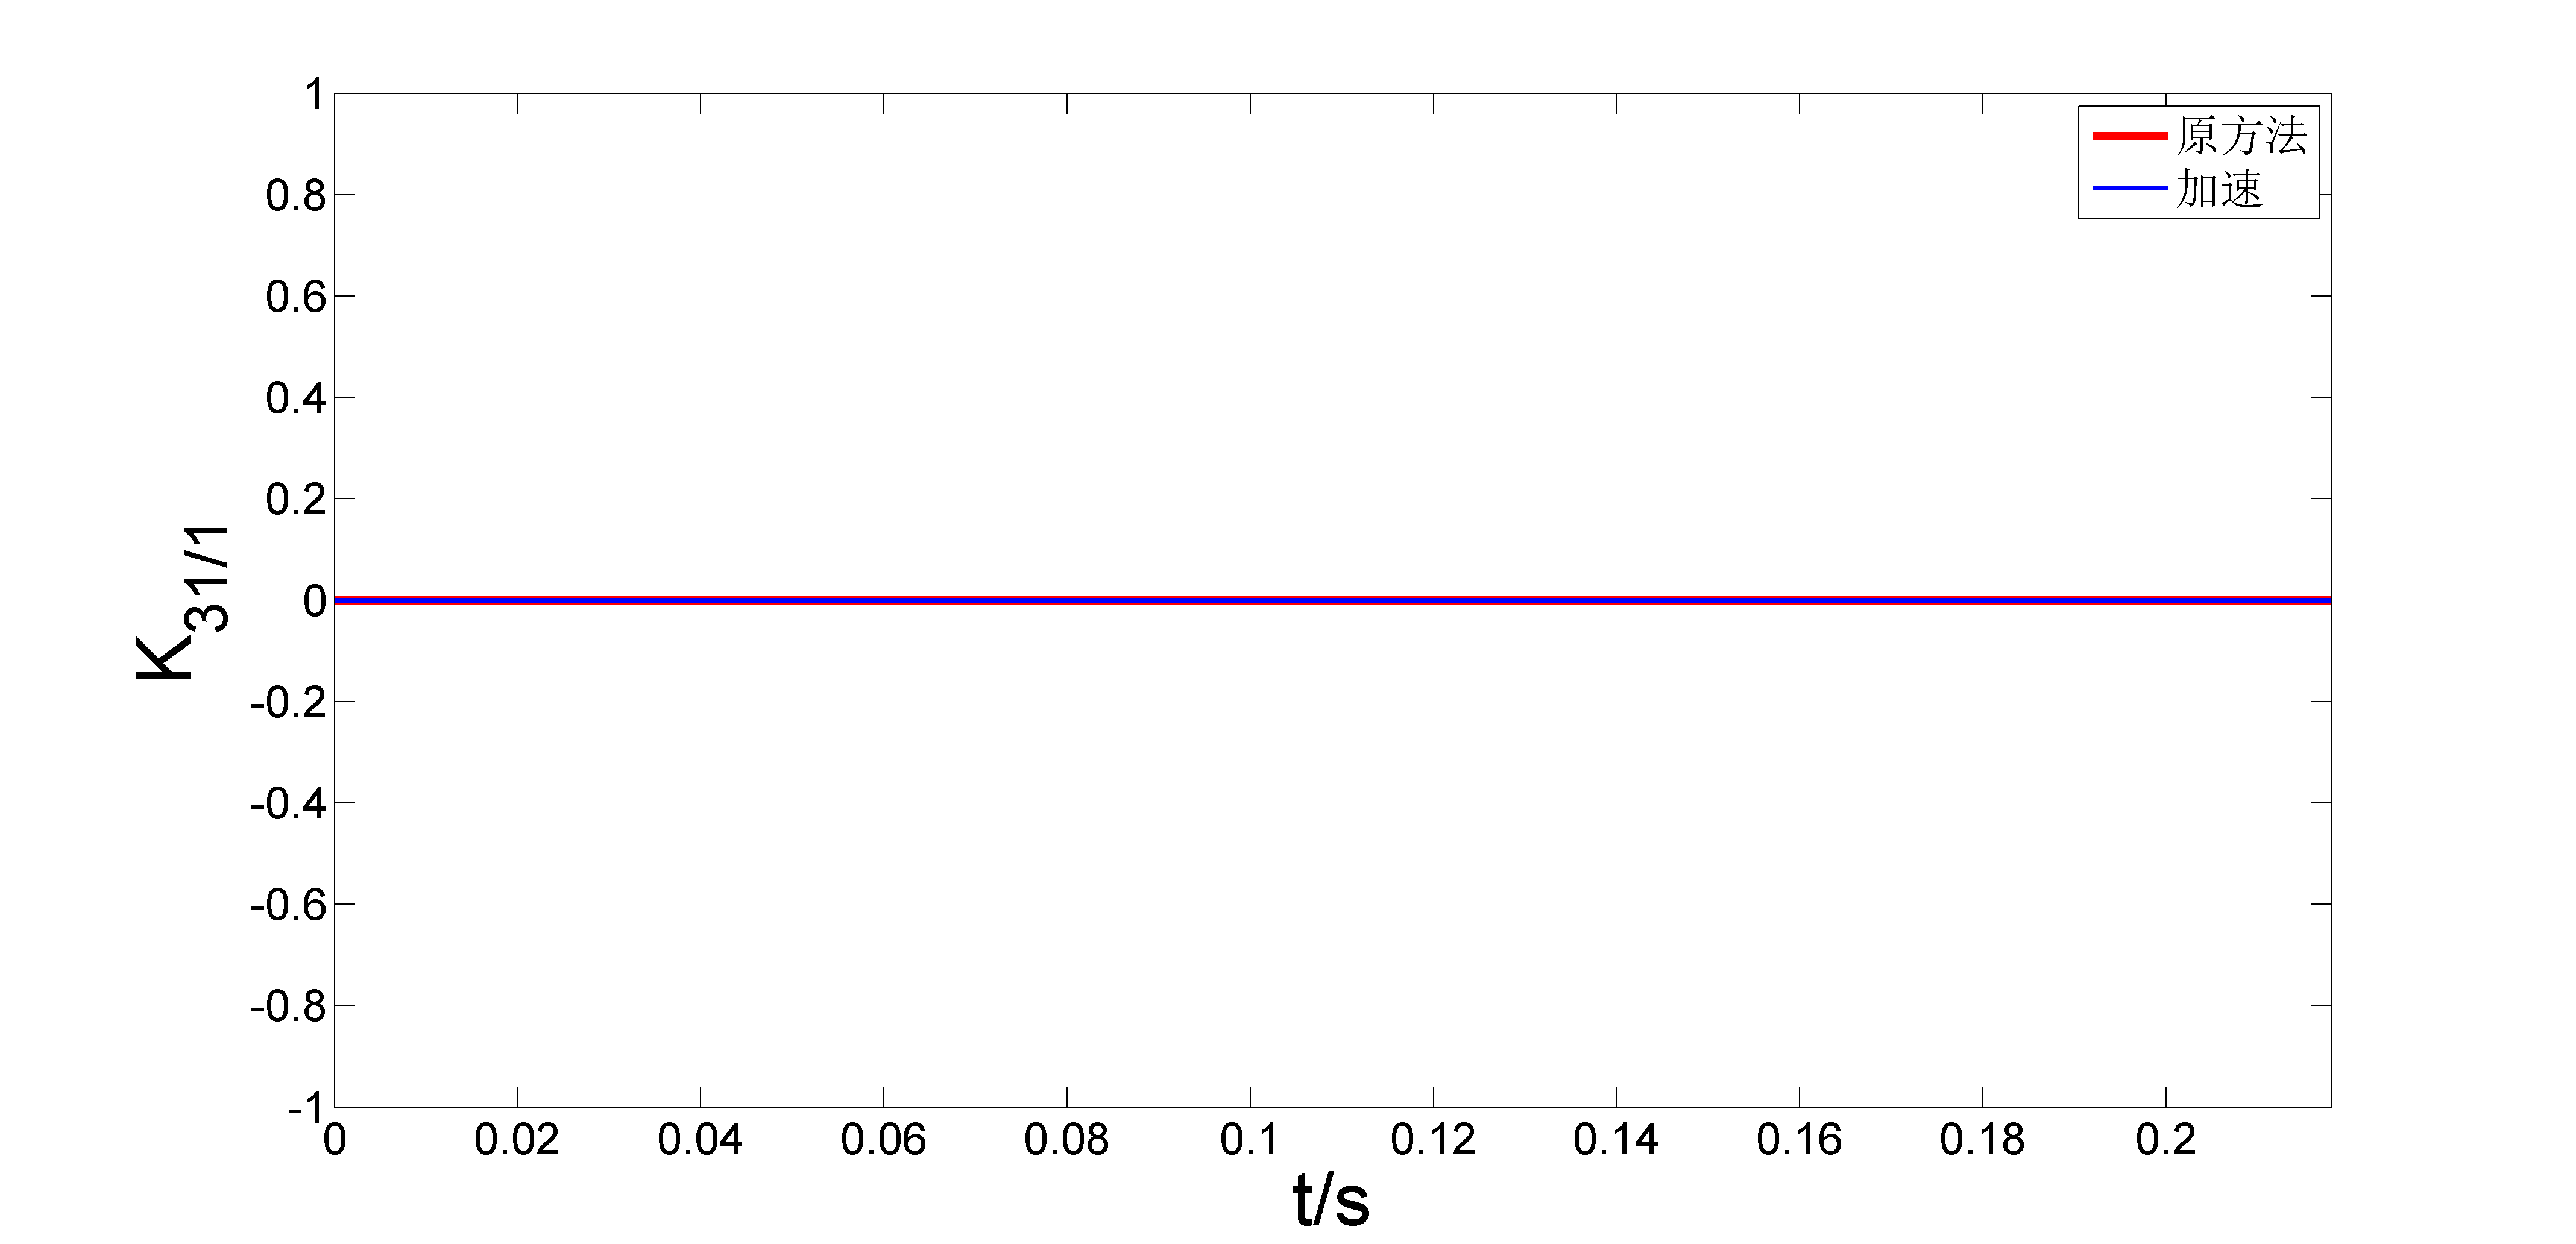
\includegraphics[width=0.5\linewidth]{L311_1_6.png}}
  % \subfigure[]{
  % 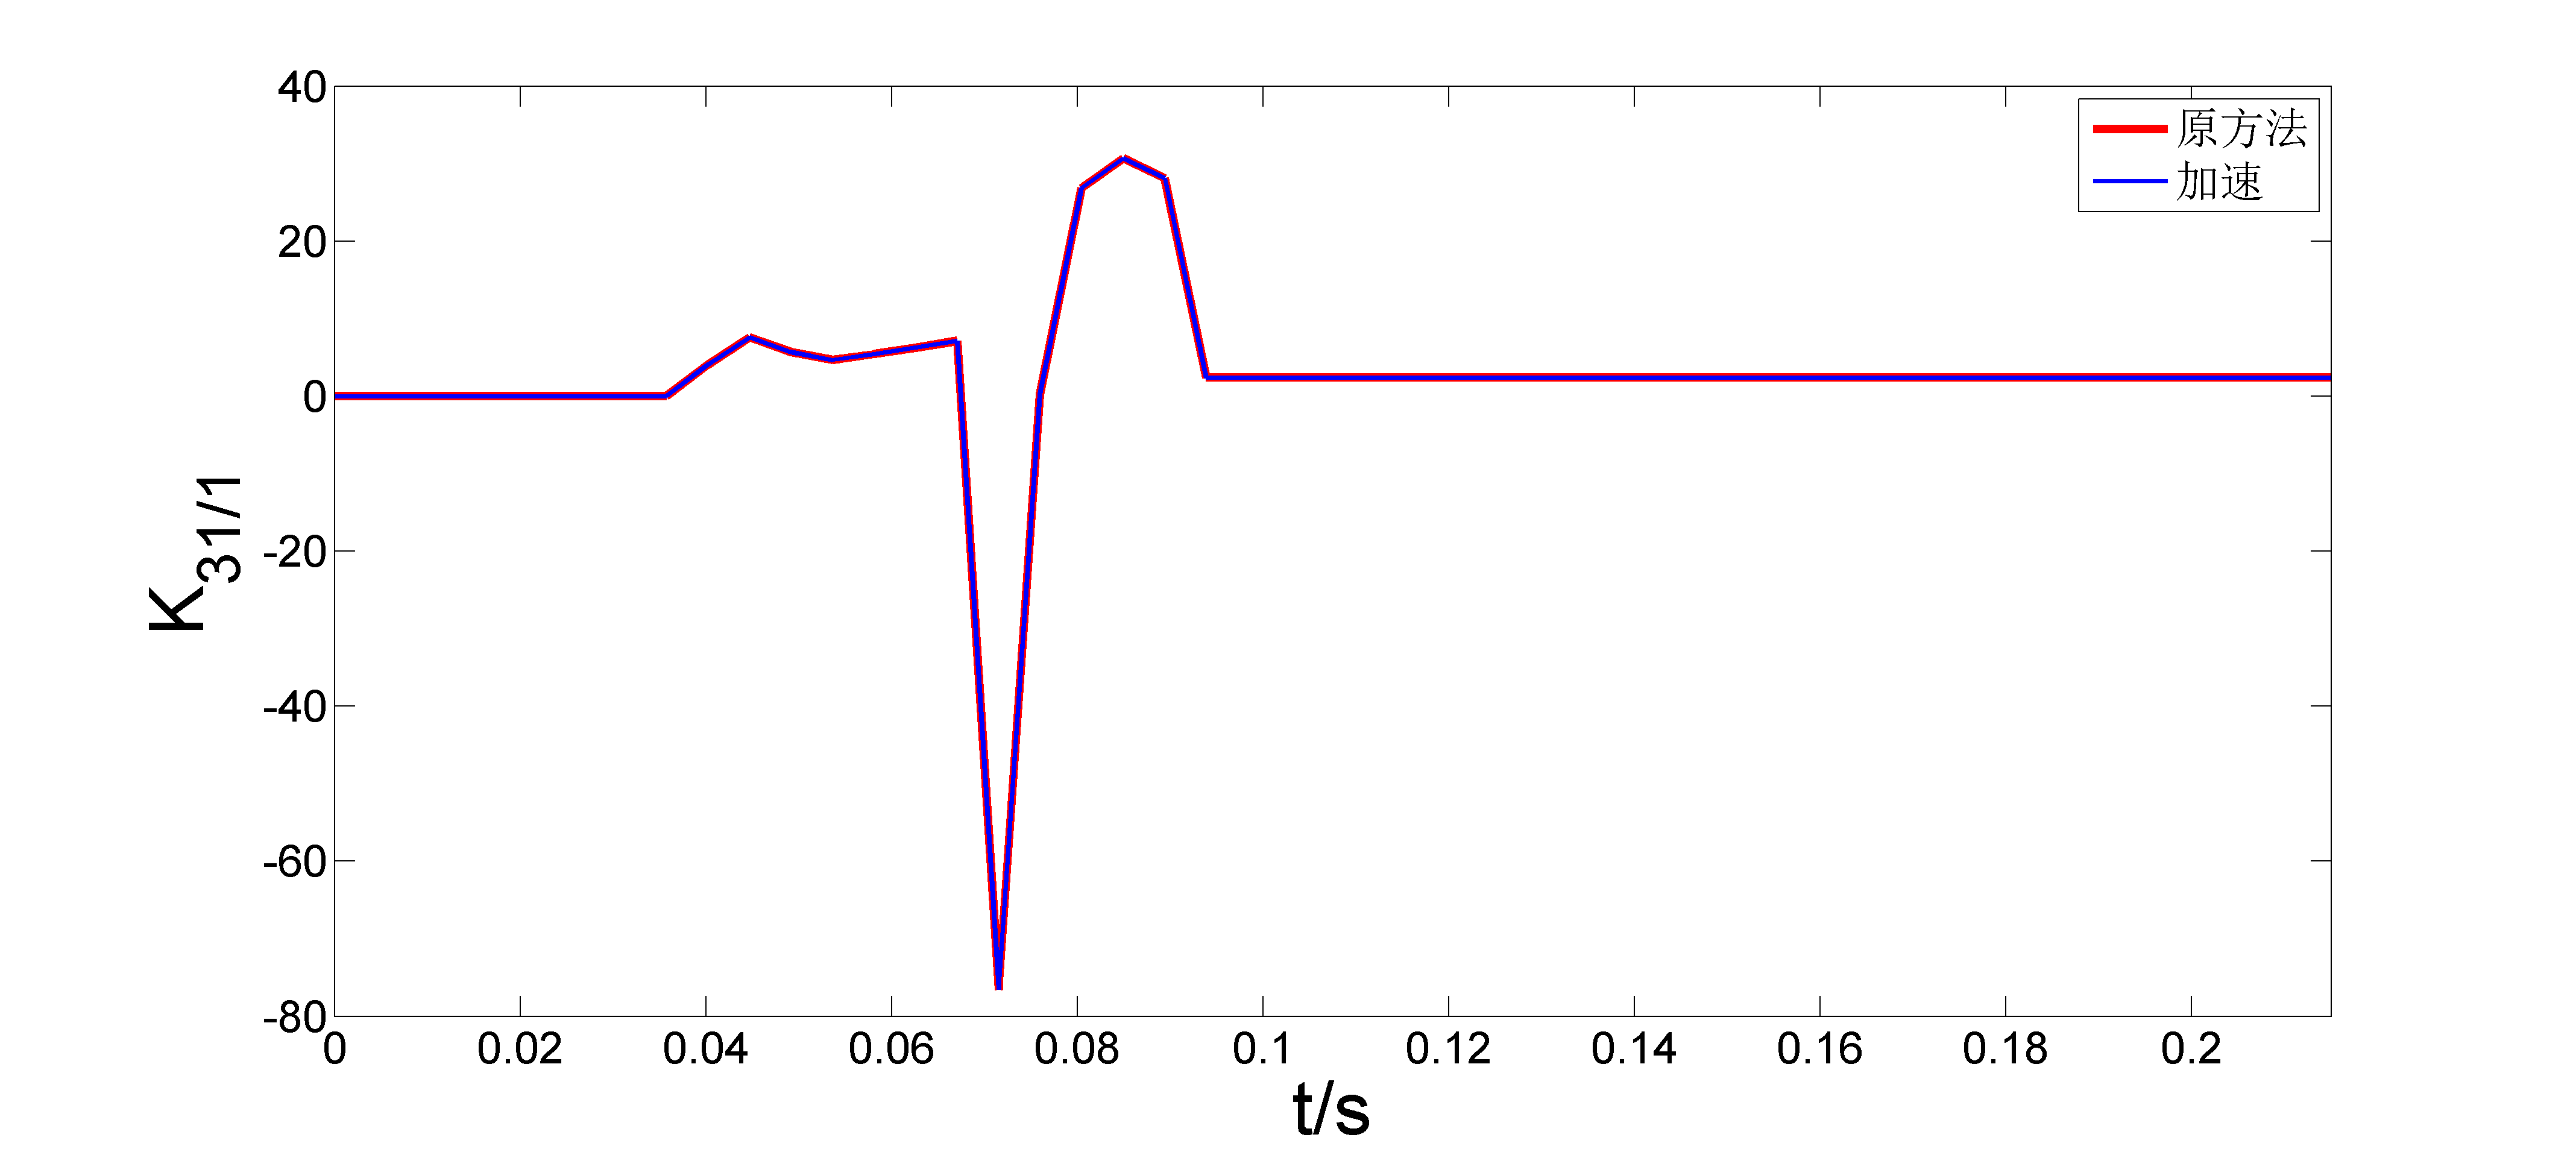
\includegraphics[width=0.5\linewidth]{L311_1_150.png}}
   %\subfigure[]{
   %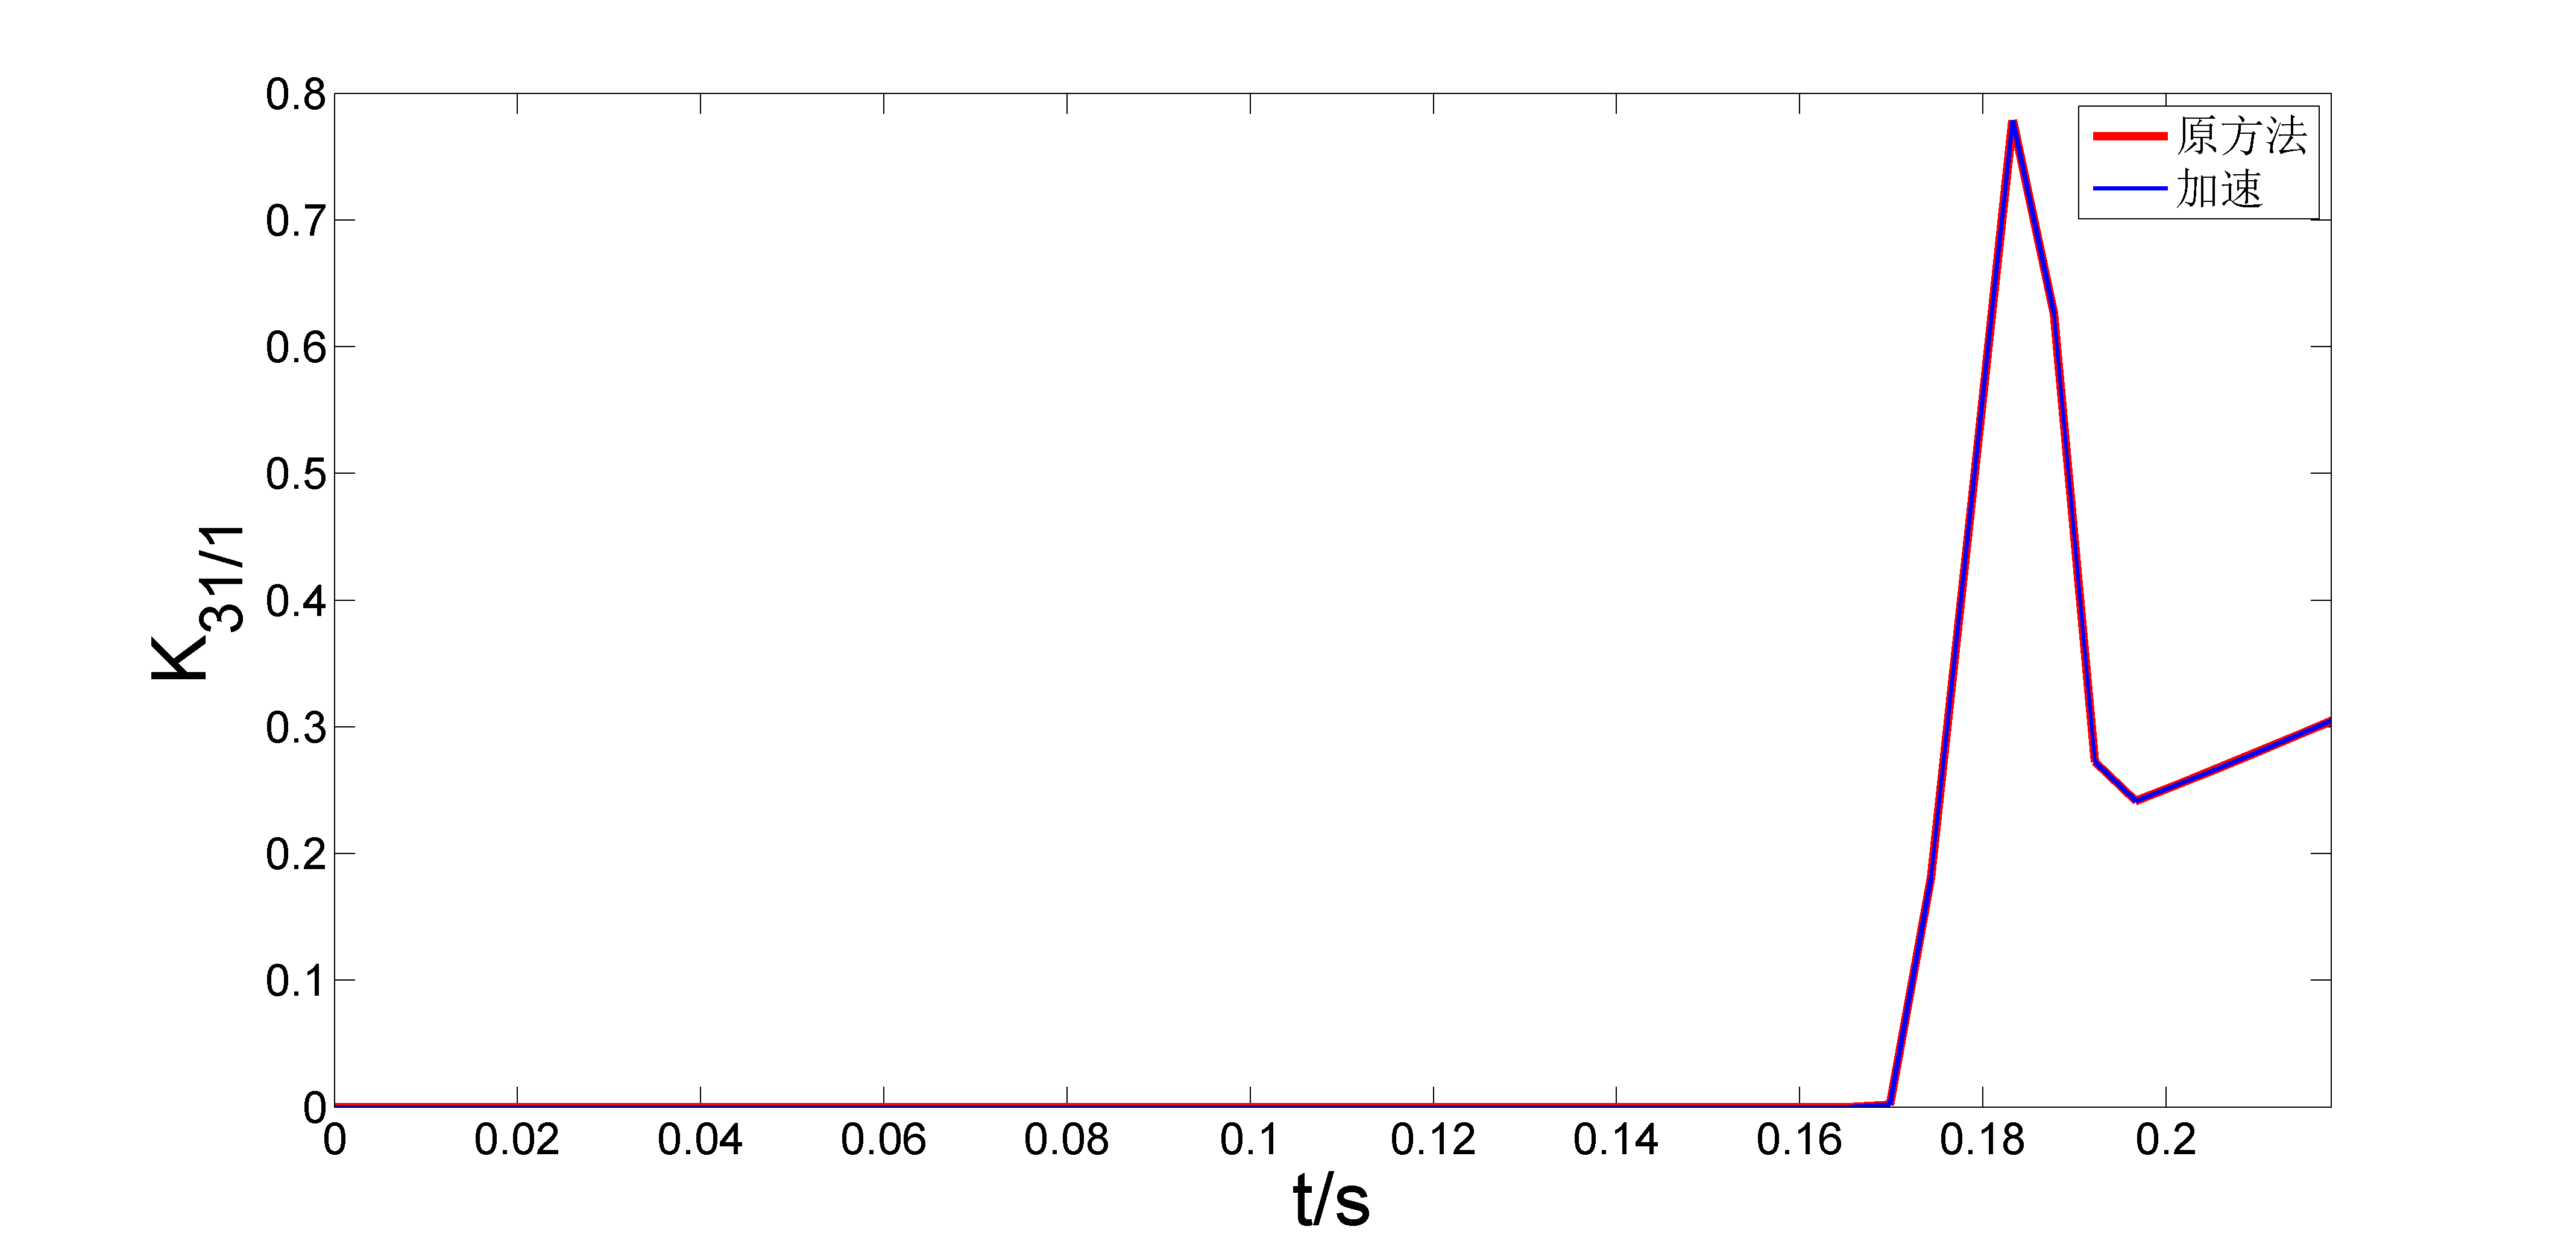
\includegraphics[width=0.5\linewidth]{L311_1_200.png}}
  % \caption{\scriptsize good job}
  %\label{2}
 %\end{figure}

 \begin{figure}[htb]
  \centering
  \begin{subfigure}[b]{0.45\linewidth}
    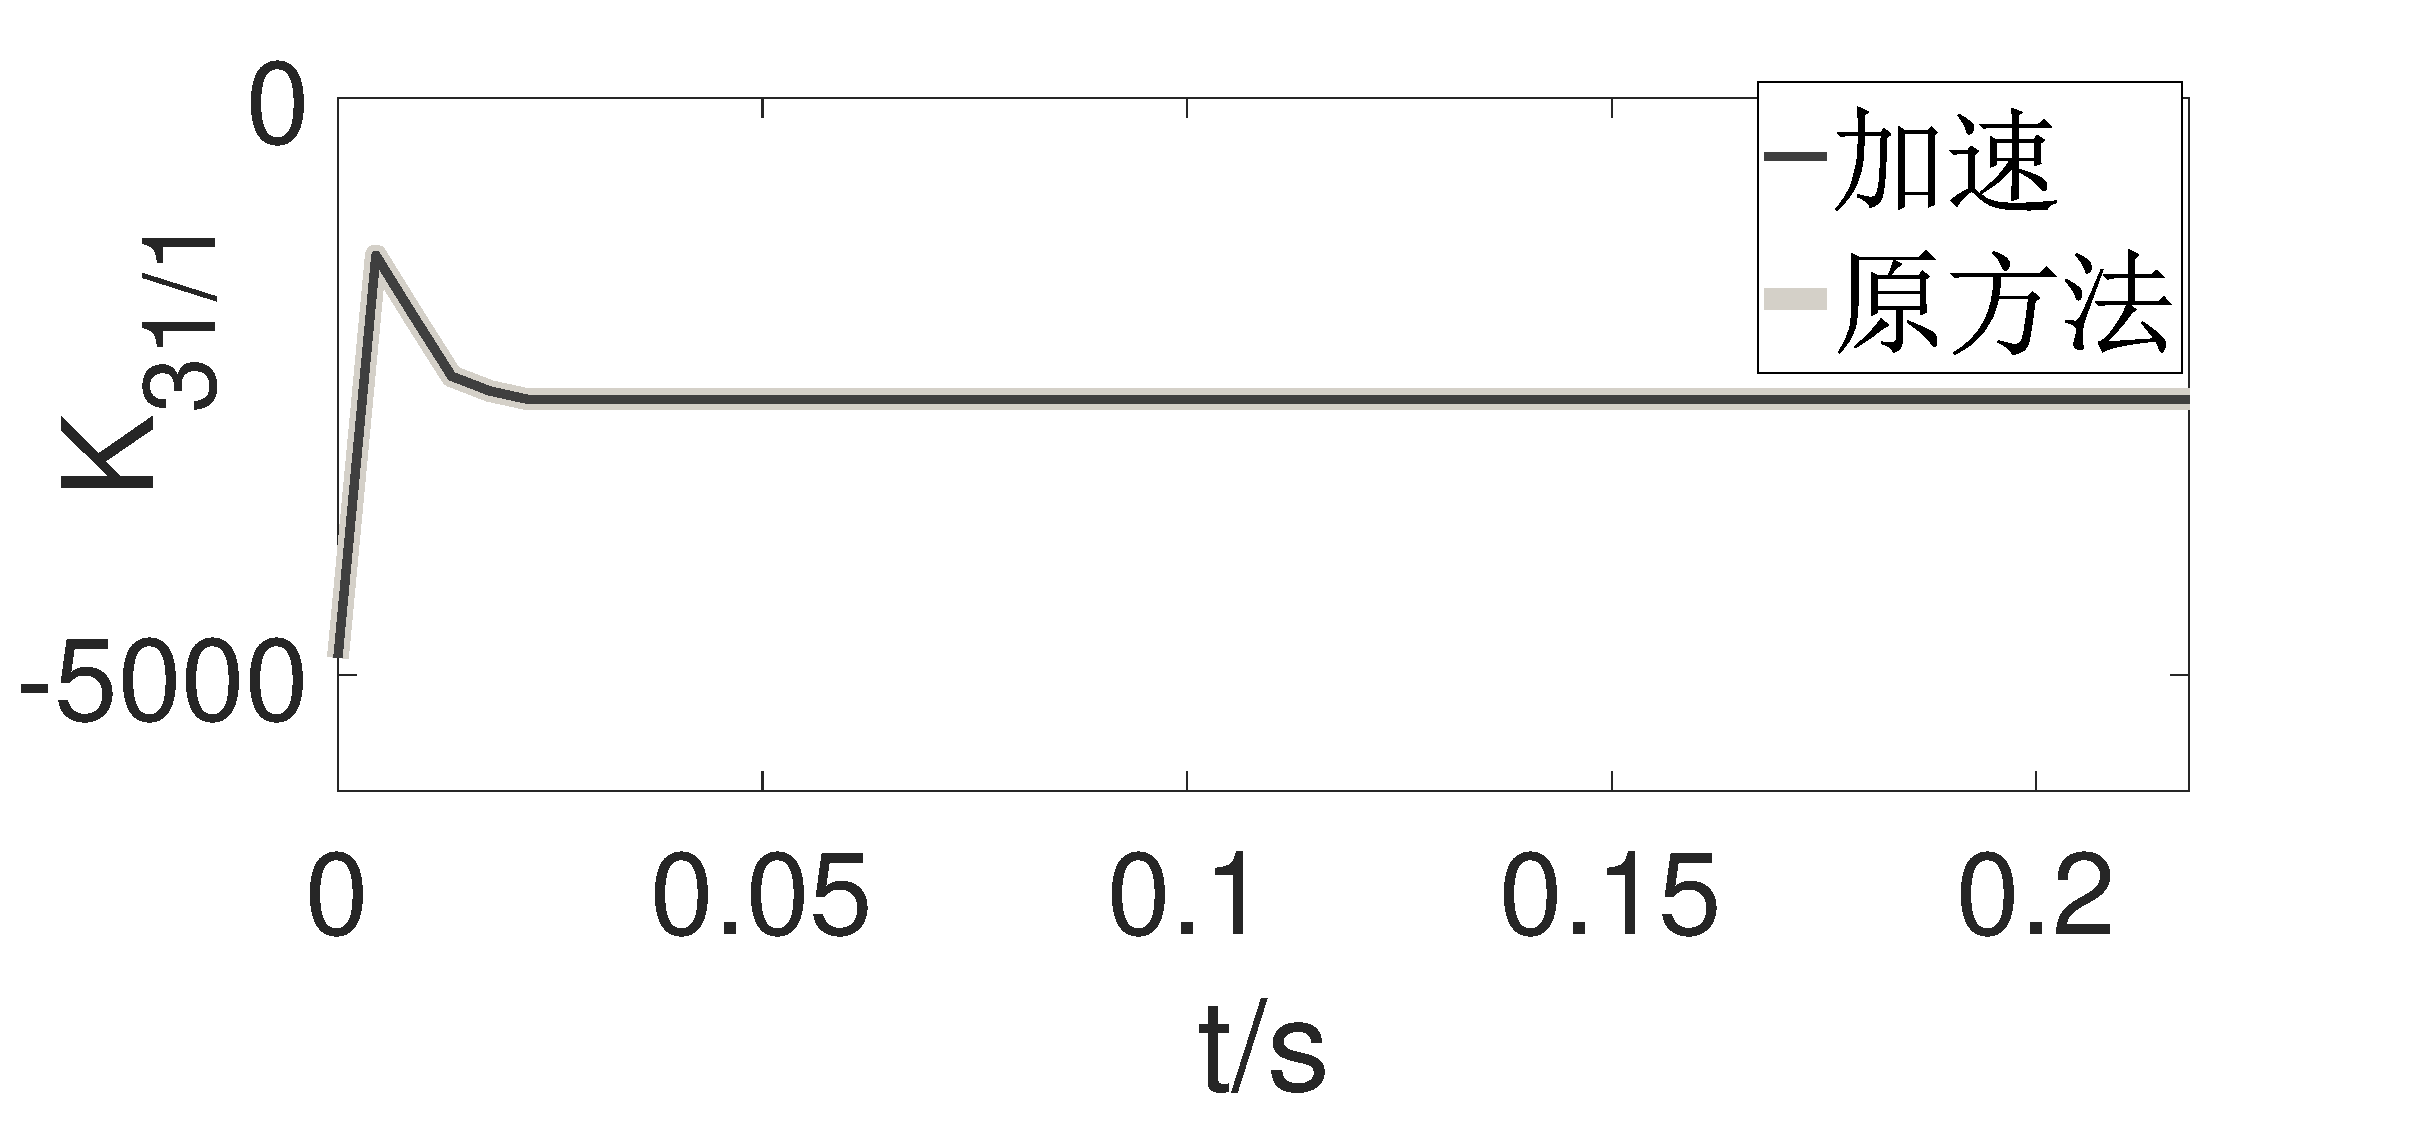
\includegraphics[width=\linewidth]{L311_1_1.eps}
    %\label{a}
    \caption{单元1对单元1的影响}\label{fig:danyuan1}
  \end{subfigure}
  \begin{subfigure}[b]{0.45\linewidth}
    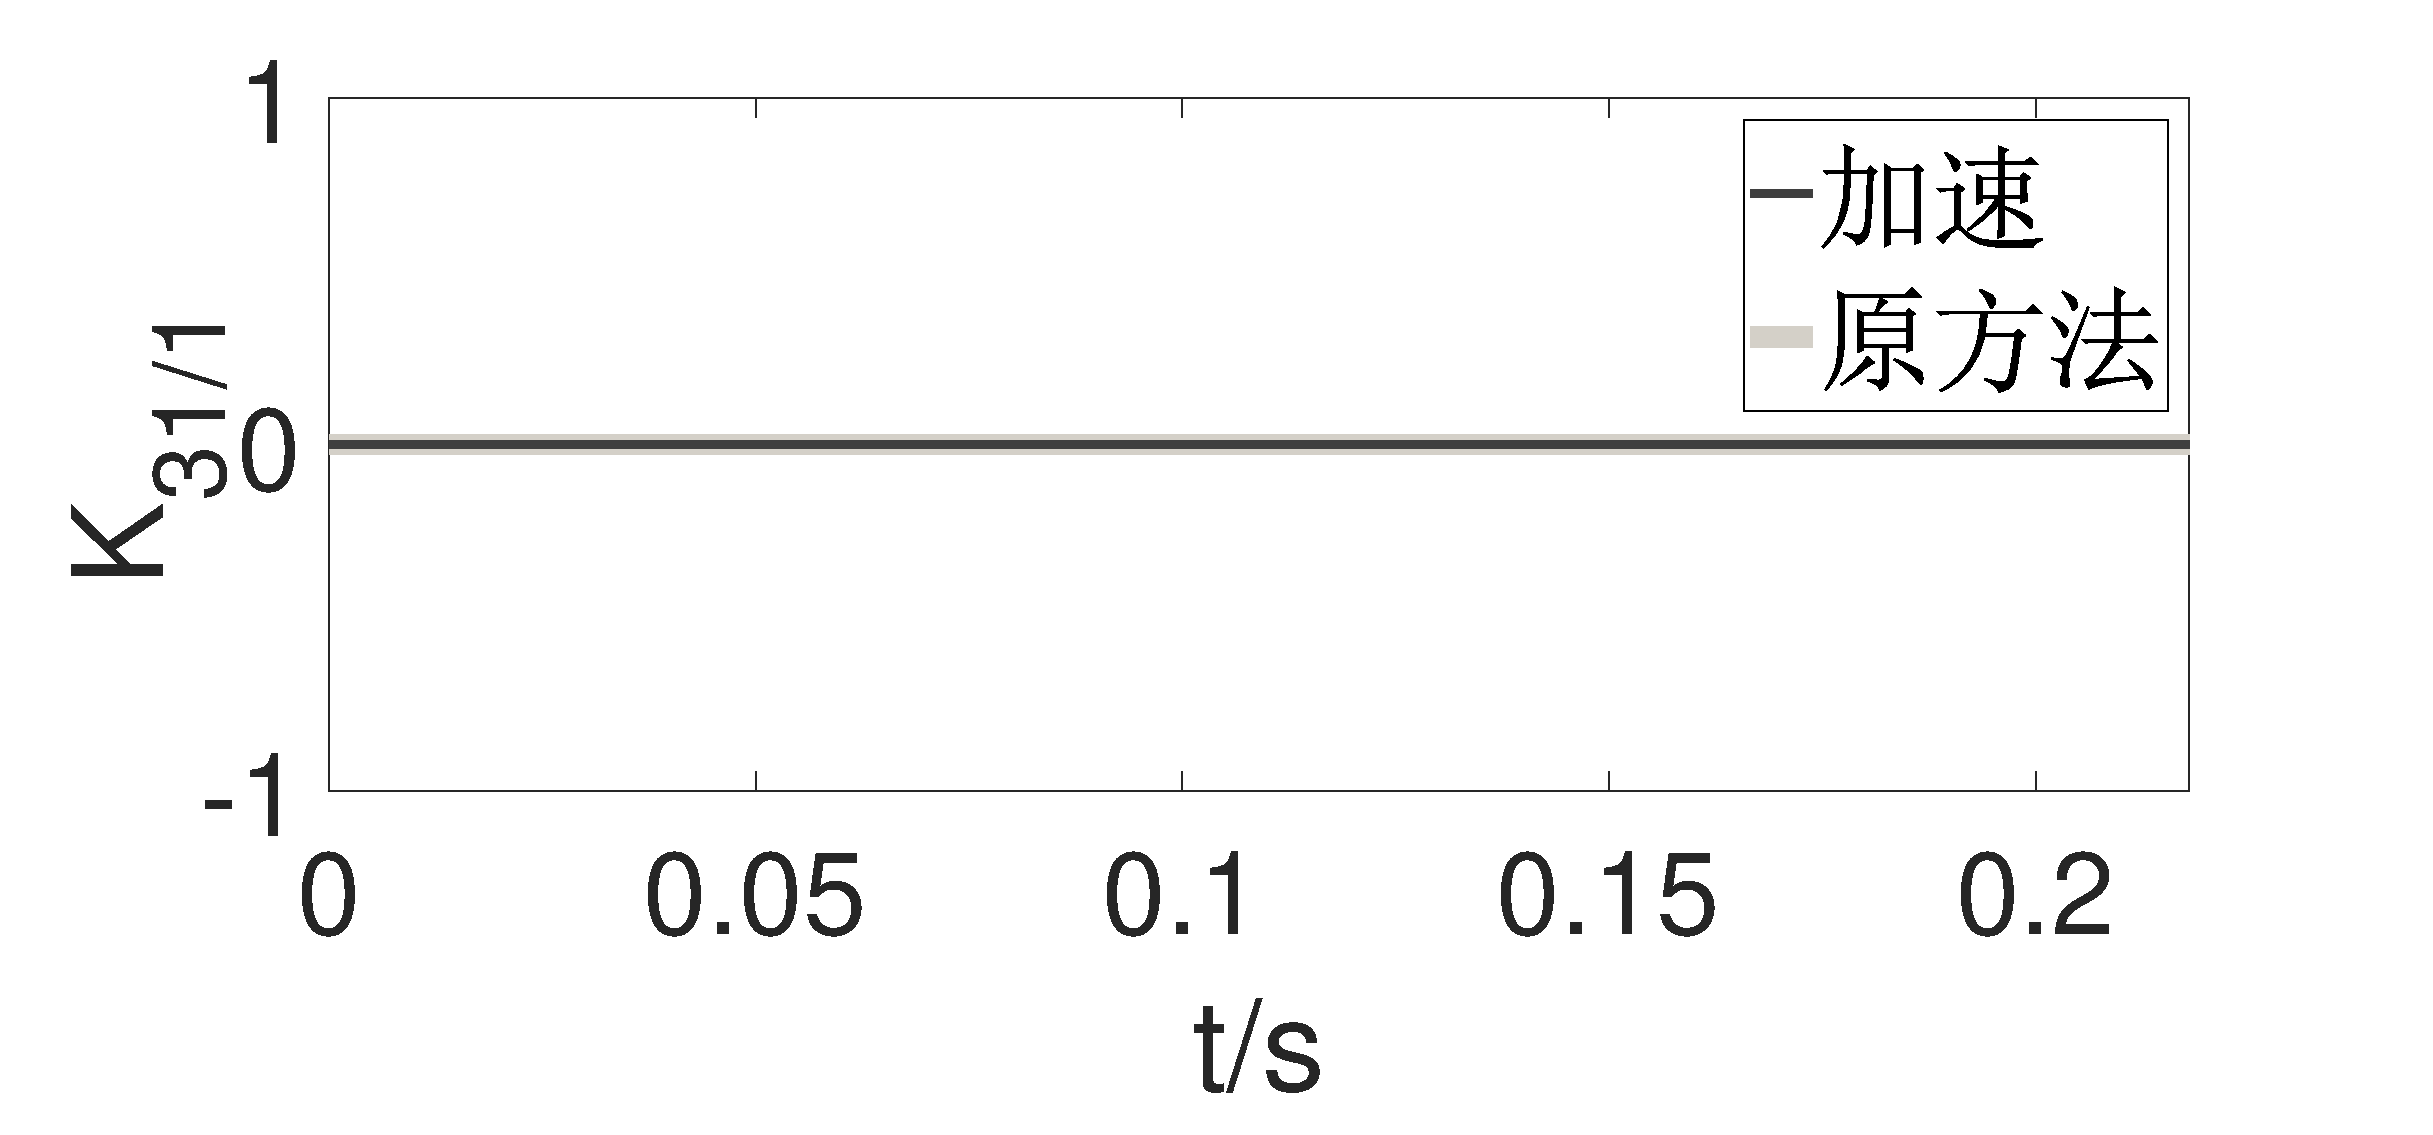
\includegraphics[width=\linewidth]{L311_1_6.eps}
    \caption{单元1对单元2的影响}\label{fig:danyuan2}
  \end{subfigure}
  \begin{subfigure}[b]{0.45\linewidth}
    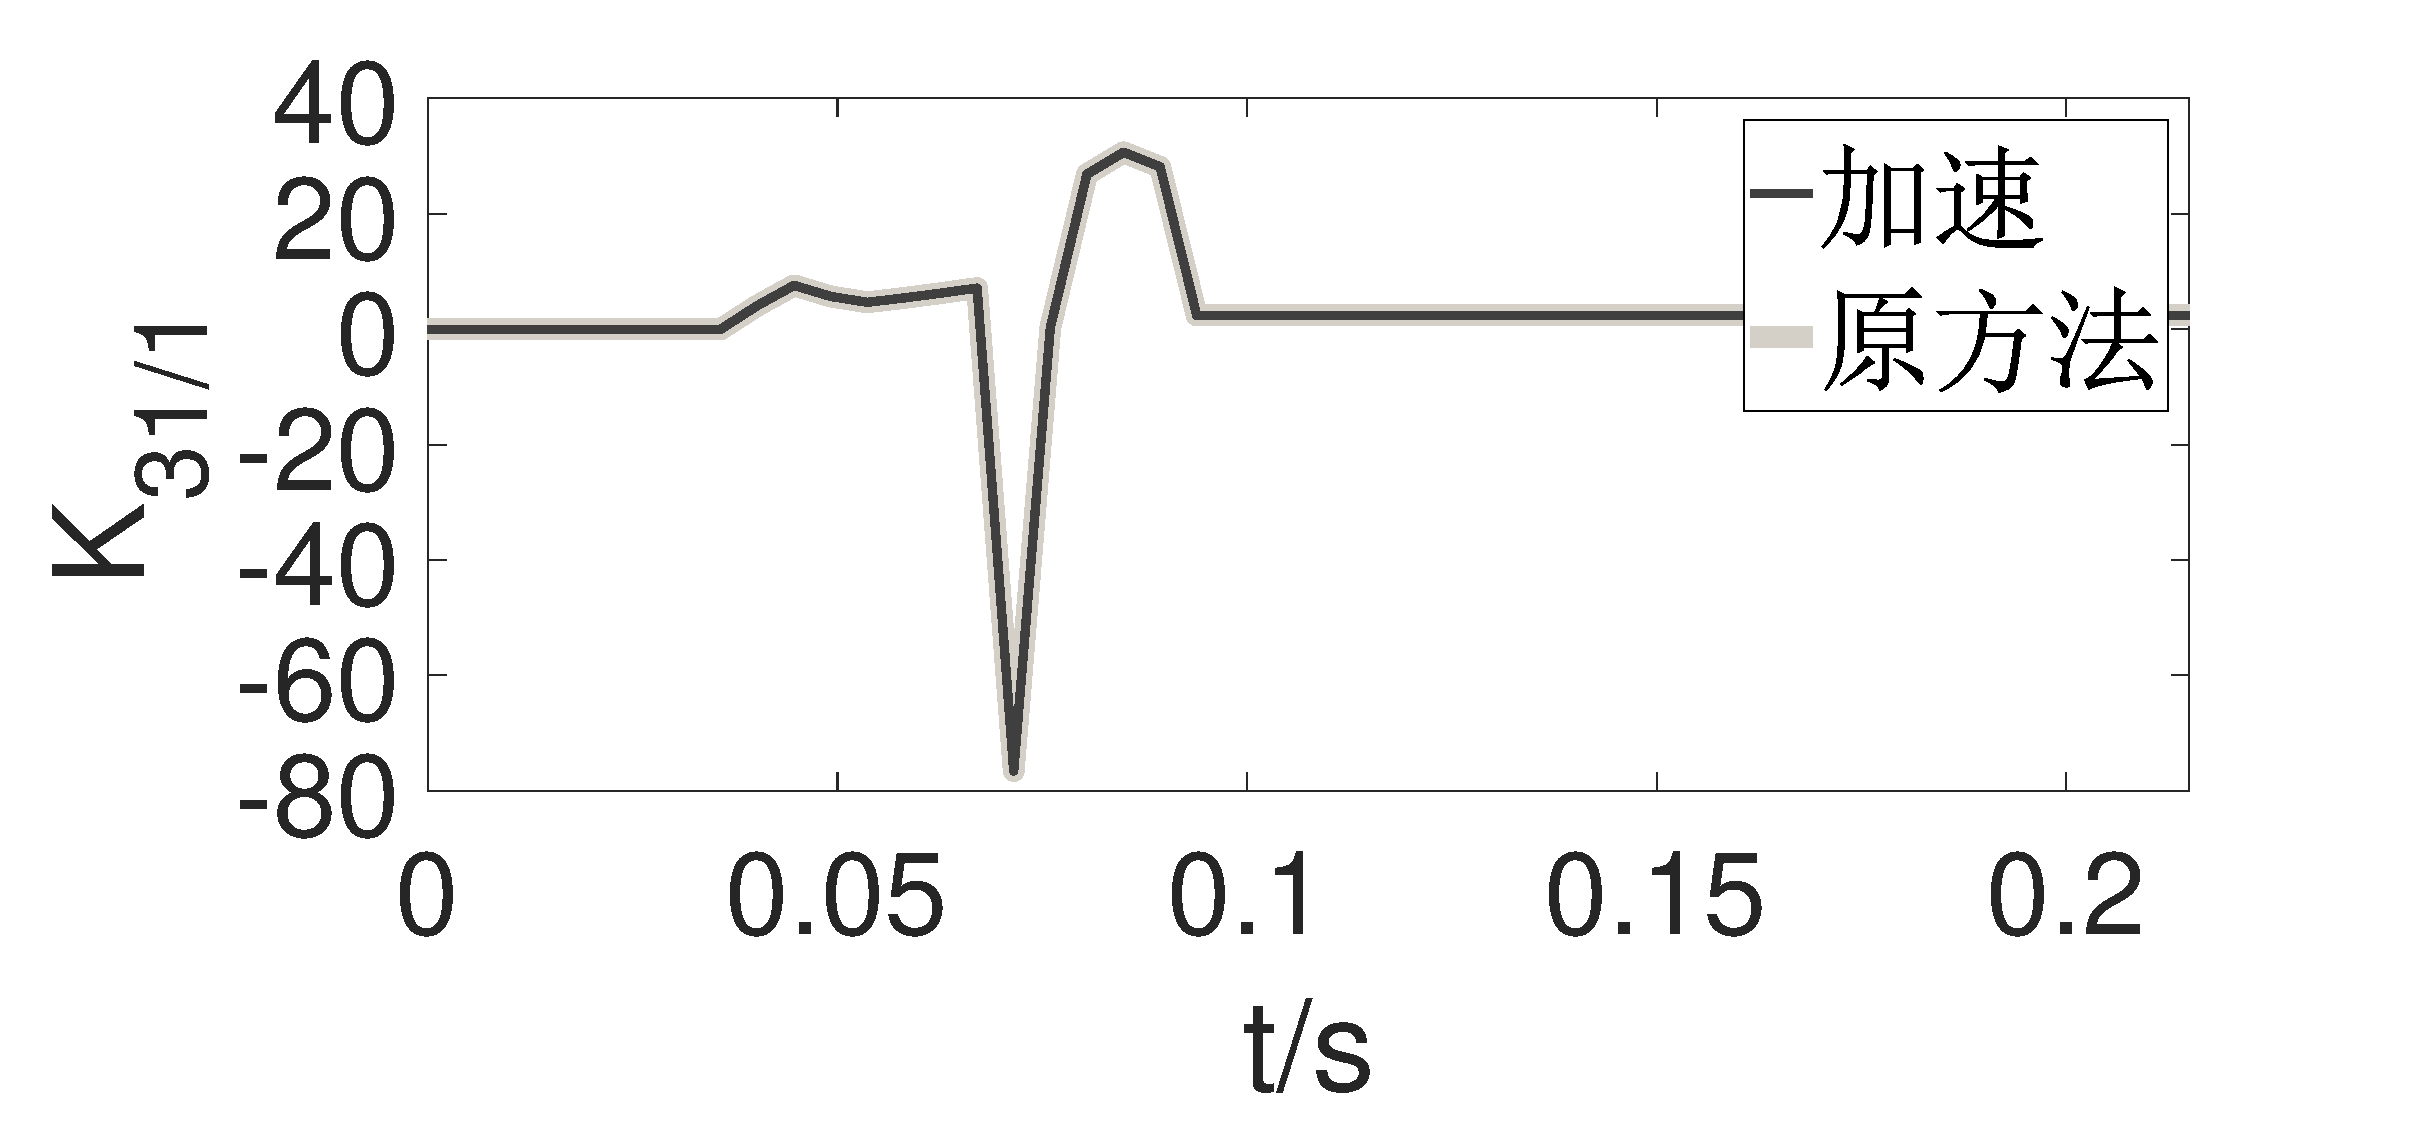
\includegraphics[width=\linewidth]{L311_1_150.eps}
    \caption{单元1对单元3的影响}\label{fig:danyuan3}
  \end{subfigure}
  \begin{subfigure}[b]{0.45\linewidth}
    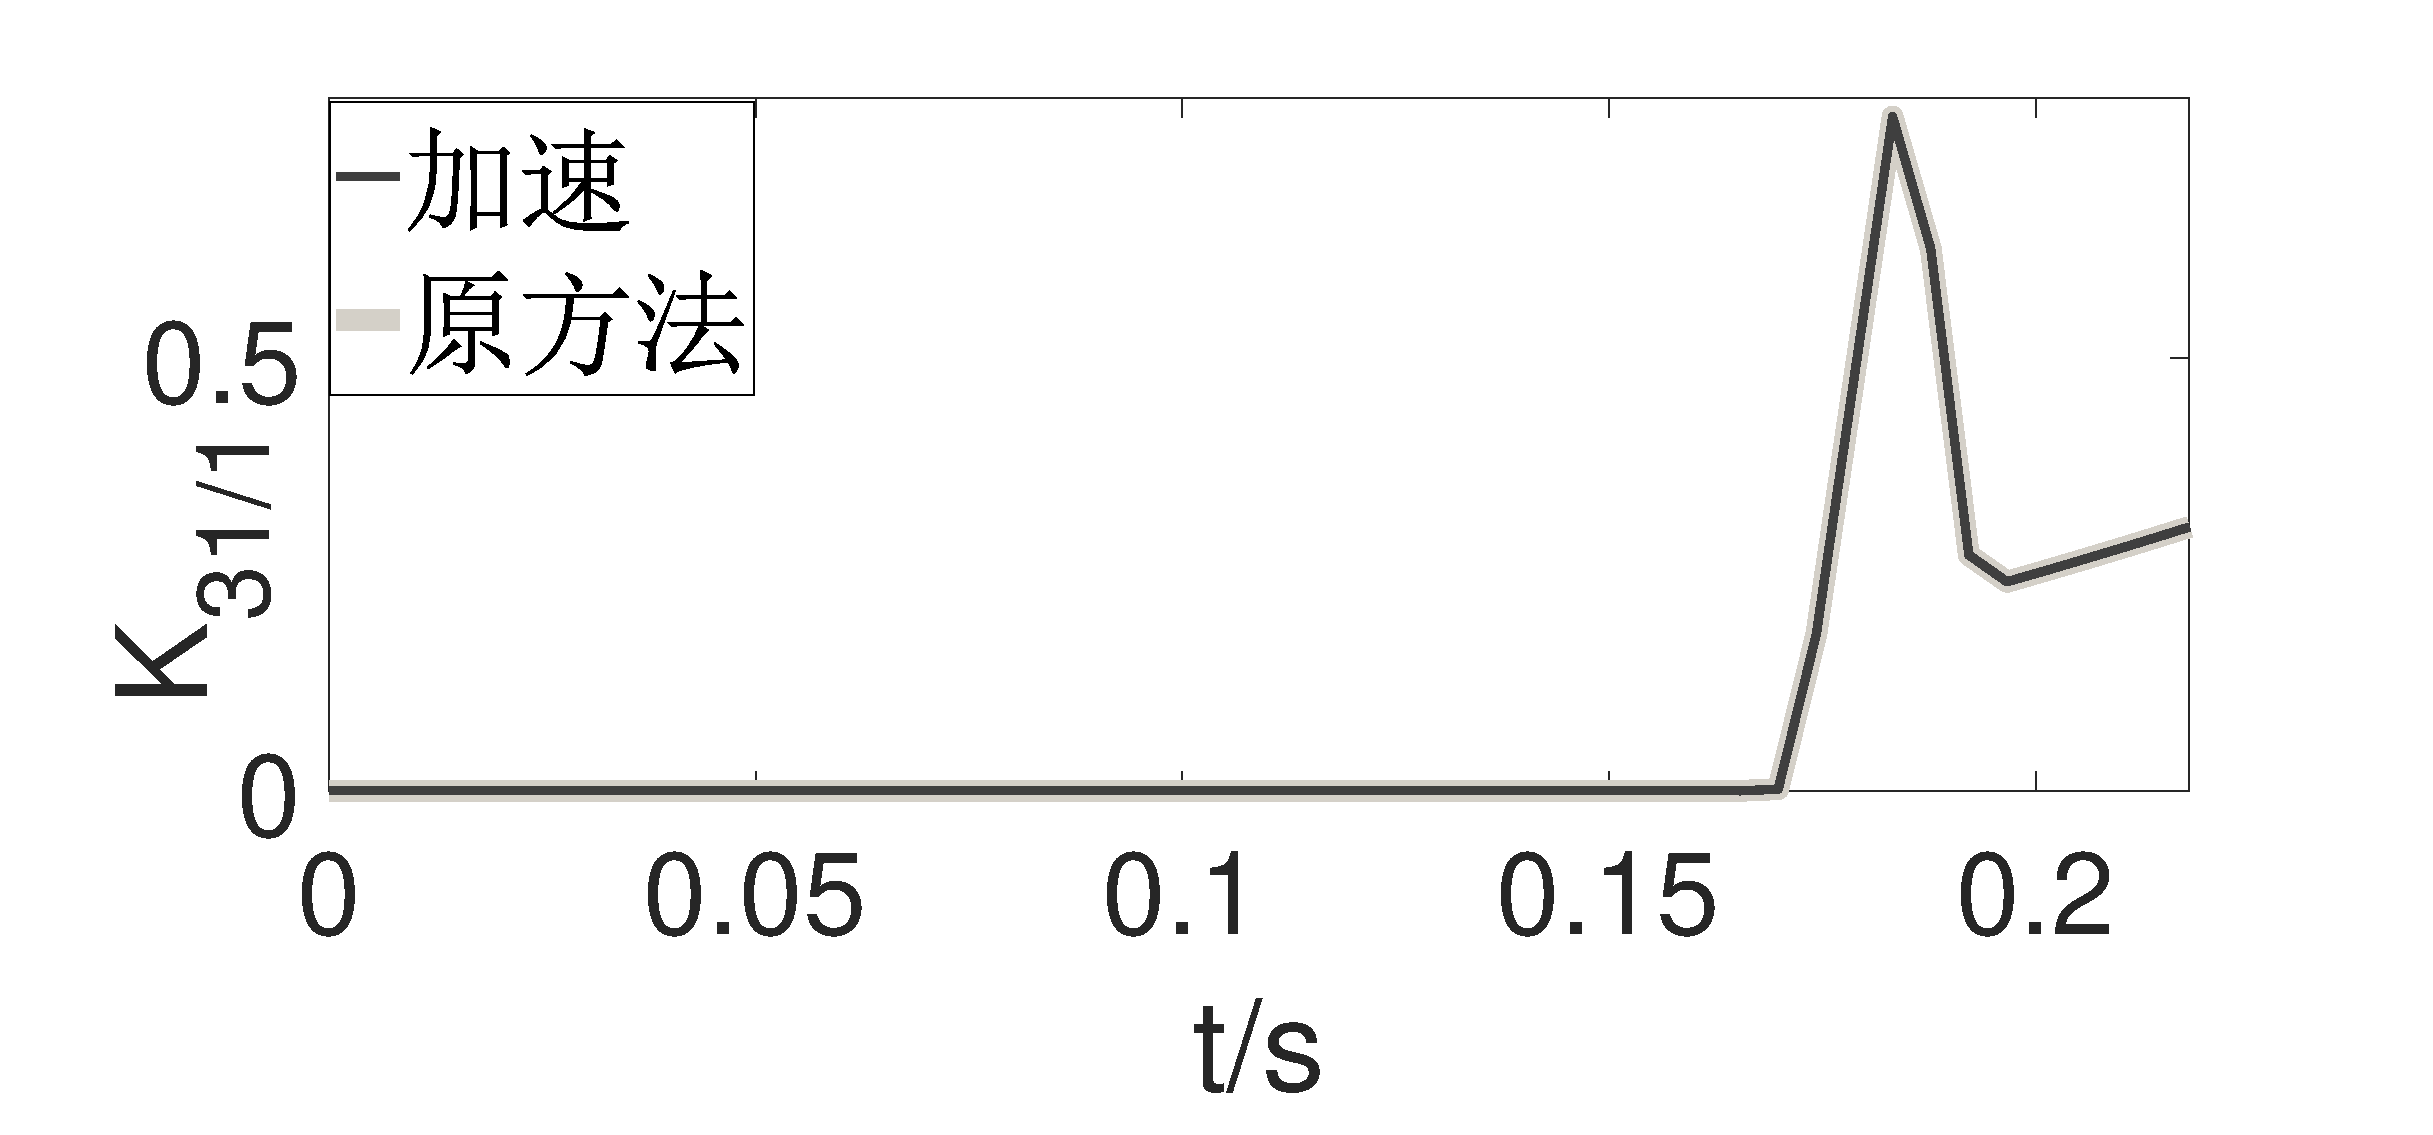
\includegraphics[width=\linewidth]{L311_1_200.eps}
    \caption{单元1对单元4的影响}\label{fig:danyuan4}
  \end{subfigure}
  \caption{积分核随时间变化图}\label{fig:demenstrate}
\end{figure}
\\

\begin{comment}
 \begin{table}
\centering  
\caption{模型坐标} \label{zuobiao} 
\begin{tabular}{|c|c|c|c|}
 \hline
顶点A&顶点B& 顶点C& 三角形\\
 \hline
(1.9194,0.5440) & (2.0000,0.4526) & (2.0000,0.5440)& 三角形1 \\
 \hline
(2.0000,0.4526) & (1.9194,0.5440) & (1.8890, 0.4525)& 三角形2\\
 \hline
(1.8888, 0.2703) & (1.8243, 0.3614) & (1.7805, 0.2709)& 三角形3\\
 \hline
( 1.0506,1.0000) & ( 1.1018,0.9079) & ( 1.0506,1.0000)& 三角形4\\
 \hline
\end{tabular}\\
\end{table}
\end{comment}
\indent 我们可以发现,加速计算后的结果和~Feng and Zhang(2017)~原有的公式计算的结果是一样的。同时,可以看出,利用分区的处理办法,能极大的提高计算的效率。如图~\ref{fig:danyuan1}~所示,该情况为三角形1对自身应力影响的积分核(也称该单元为共位单元)。对于~$t_c$~之后的积分核,采用分区处理的办法是不用计算这个部分的,可以得到计算效率提高 91\%。如图~\ref{fig:danyuan2}~所示此积分核值为0。 若采用原有方法,需要计算整个过程。而采用分区处理的办法,判断地震波传播仍处于初始区中,则可以直接得到该部分的所有积分核值都为0.计算的效率提高约为百分之百。对于,图~\ref{fig:danyuan3},图~\ref{fig:danyuan4}~仍然能得到利用分区法能够加速计算积分核的结论。因此,我们可以认为,在保证正确率的同时,分区处理积分核方法能极大的提高计算效率。\\
    \indent 至此本章通过数值推导与分析,得到了分区域计算积分核的办法,实现了计算效率的提高,并且通过~Matlab~编程对加速后的方法进行正确性检验。下一章中将用~Matlab~编程实现该方法,并对具体算例进行研究。

		
\section{模型评估与选择}

 \indent 通常上我们把机器学习器在训练集上的误差称为训练误差(training error)或者经验误差(generalization error),在新样本上的误差称为泛化误差(generalization error)。原则上最终人们希望得到一个泛化误差小的模型,也就是模型在面对没有出现在训练集中的新数据能有优异的预测性。但事实上我们并不知道新的样本是什么样的,集体到本问题中对于还未发生的地震我们并不知道其发震断层的模型,也不清楚震源附近的介质模型,实际上能做的是努力使训练误差最小化。在很多情况下,我们都可以使模型学习到一个在训练集上表现很好,经验误差很小的机器学习器。甚至对于整个训练数据集没有错误分类达到100\%准确率或者完全没有预测误差的学习器,但这样的机器学习器在绝大多数的情况下并没有好的泛化能力。
 
 \indent 我们核心的训练目标是在新样本上表现卓越。为了达到这个目的,我们要使模型从训练数据中尽可能的学习到问题"内在规律",这样才能使模型在遇到实时地震台站数据记录时做出正确判别。当学习器把训练样本学得“太好”时,很可能已经把训练样本自身的一些特点当作了所有潜在样本都会具有的一般性质,这就很会导致泛化性能下降。此现象在机器学习中称之为"过拟合"(overfitting),与之相对应“欠拟合”(underfitting),这是指对训练样本的一般性质尚未学习好。图2.4直观展示了过拟合和欠拟合的区别。
 
\begin{figure}[ht]
  \centering
  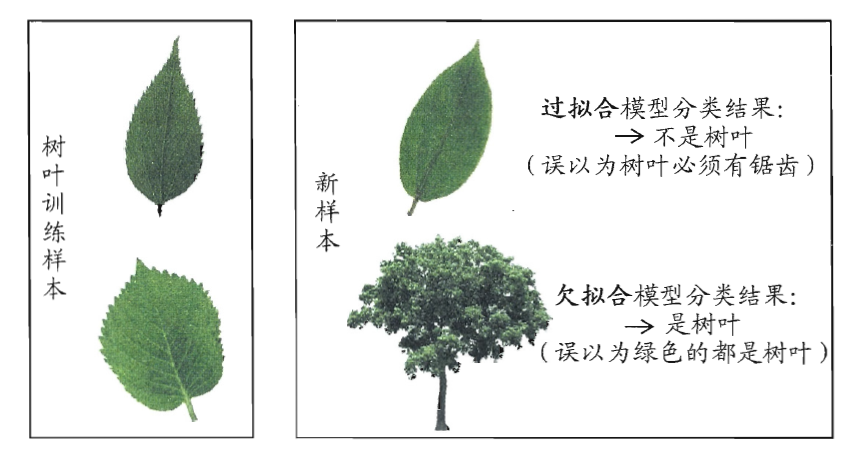
\includegraphics[width=\linewidth]{img/fitting.jpg}
  \caption{过拟合、欠拟合的直观类比}\label{fig:yinglimoxin}
\end{figure}

 \indent 机器学习模型往往着力于解决的过拟合问题。在实践中往往有多种原因导致过拟合问题的出现。较为常见的情况有,因模型学习能力过于强而导致训练数据集中所包含的非一般特性都被模型学习到。而欠拟合则通常是由于模型复杂度低下和学习能力不足造成,例如在神经网络学习中采取增加模型网络深度和增加训练轮数可以克服欠拟合问题。与之相对的过拟合问题是机器学习面临的核心阻碍,在各类具体的机器学习模型中都有各自机制来应对,但原则上过拟合问题是不可避免的,以上的机制也只能部分的缓解过拟合问题。
 
 \indent 一般的可以通过实验测试来对机器学习模型的泛化能力进行评估,同时完成对模型参数的选择。故我们需要一个有别于训练数据集(training set)的测试数据集(testing set)。若假设测试数据集中新样本也是从真实事件分布中独立同分布采样而得到,同时测试数据集与训练数据集互斥度越大越佳,这就意味着测试数据集中样本尽量没有出现过在训练过程中。在这种假设下我们可以使用测试数据集的测试误差(testing error)作为模型对于真实泛化能力的估计。机器学习模型对于新样本的分别能力越出众,则其在测试数据集上的误差越小。对于一个包含m个样本的数据集$D=\left\{\left(\boldsymbol{x}_{1}, y_{1}\right),\left(\boldsymbol{x}_{2}, y_{2}\right), \ldots\right.\left(\boldsymbol{x}_{m}, y_{m}\right) \}$,通常从D中适当的分出训练集S和测试集T两个互斥的子集。
 
 \subsection{留出法训练方法}
 \indent 常见朴素的思想以留出法为框架。通常的做法为直接将全数据集D划分为互斥的两个集合,这两个集合S、T满足,$D=S \cup T, S \cap T=\varnothing$. ~即使用训练数据集S上进行模型训练,随后在测试数据集T上进行模型泛化能力评估。